% Einfache LaTeX-Vorlage für Arbeiten am Lehrstuhl Kranzlmüller / MNM-Team
% - optimiert für die Arbeit mit gängigen LaTeX-Editoren
% - funktioniert ohne Makefile und Anpassungen der LaTeX-Verzeichnisstruktur
% - verwendet Komaskript für ein (nach europäischen Gepflogenheiten) schöneres Layout
% 
% v1, 2007 (Michael Brenner)
% Diese Version: v1.1, 2012 (Michael Brenner)


%%%enabledeprecatedfontcommands for less errors
\documentclass[enabledeprecatedfontcommands,bibliography=totoc,listof=totoc,BCOR=5mm,DIV=12]{scrbook} 

%\usepackage{bibgerm}       % deutsche Literaturverzeichnisse
\usepackage[utf8]{inputenc}
 % Umlaute im Text
\usepackage{graphicx} % Einfügen von Grafiken  - für PDF-Latex: .pdf und .png (.jpg möglich, sollte aber vermiedenwerden)
\usepackage[hyphens]{url}          % URL's (z.B. in Literatur) schöner formatieren
\usepackage{hyperref} % sorgt für für Hyperlinks in PDF-Dokumenten
\usepackage{rotating}
\usepackage{longtable}
\usepackage{verbatim}
\usepackage{amsmath}
\usepackage{enumitem}
\usepackage{amsfonts}
\usepackage{amssymb}
\usepackage{float}
\usepackage{placeins}
\usepackage{subcaption}
\usepackage[table,xcdraw]{xcolor}
\usepackage{xcolor}
\definecolor{gruen}{RGB}{27,158,119}
\definecolor{orangedunkel}{RGB}{217, 95, 2}
\definecolor{lila}{RGB}{117, 112, 179}
\usepackage{booktabs}
%%Adds more space bewteen row
\renewcommand{\arraystretch}{1.2} 
\usepackage{listings}
\usepackage{tikz}
%%%%%%%%%%%%

%%%%%%%%%%%%%%%%
\usetikzlibrary{calc,trees,positioning,arrows,chains,shapes.geometric,%
    decorations.pathreplacing,decorations.pathmorphing,shapes,%
    matrix,shapes.symbols}

\tikzset{
>=stealth',
  punktchain/.style={
    rectangle, 
    rounded corners, 
    % fill=black!10,
    draw=black, very thick,
    text width=10em, 
    minimum height=3em, 
    text centered, 
    on chain},
  line/.style={draw, thick, <-},
  element/.style={
    tape,
    top color=white,
    bottom color=blue!50!black!60!,
    minimum width=8em,
    draw=blue!40!black!90, very thick,
    text width=10em, 
    minimum height=3.5em, 
    text centered, 
    on chain},
  every join/.style={->, thick,shorten >=1pt},
  decoration={brace},
  tuborg/.style={decorate},
  tubnode/.style={midway, right=2pt},
}
%%%%%%%%%%%%%%%%%%%%%%%%%%%%%

\graphicspath{{./Bilder/}}

\input{hyphenation} % in dieses File kommen Wörter die Latex nicht richtig trennt

\begin{document}

% ---------------------------------------------------------------
\frontmatter % Titelblätter und Erklärung jeweils spezifisch für die jeweilige Uni einbinden
    %%%%%%%%%%%%%%%%%%%%%%%%%%%%%%%
% erste Seite

\thispagestyle{empty}

\begin{center}

\vspace*{-2cm}

{\Huge INSTITUT F\"UR INFORMATIK\\[1mm]}
DER LUDWIG--MAXIMILIANS--UNIVERSITÄT MÜNCHEN\\

\vspace*{1cm}

\includegraphics[width=0.3\textwidth]{lmu_siegel}

\vspace*{2cm}

{\Large \textbf{Master's Thesis}}\\ % oder Fortgeschrittenenpraktikum, Master's Thesis, Bachelorarbeit etc.

\vspace{2.0cm}
{\Huge \textbf{Edge vs. Cloud:}}\\
\vspace*{2.5mm}
{\Huge \textbf{Deployment of Deep Learning}}\\
\vspace*{2mm}
{\Huge \textbf{Models}}\\
\vspace{1.5cm}

{\LARGE Philipp Johannes Roß} % Name des Autors

\vspace{3cm}
Draft vom \today % erleichtert den Betreuern die Zuordnung - für finale Version entfernen

\end{center}

\newpage

%%%%%%%%%%%%%%%%%%%%%%%%%%%%%%%
% zweite Seite

\thispagestyle{empty}
\cleardoublepage

%%%%%%%%%%%%%%%%%%%%%%%%%%%%%%%
% dritte Seite (Kopie der ersten)

\thispagestyle{empty}

\begin{center}

\vspace*{-2cm}

{\Huge INSTITUT FÜR INFORMATIK\\[1mm]}
DER LUDWIG--MAXIMILIANS--UNIVERSITÄT MÜNCHEN\\

\vspace*{1cm}

\includegraphics[width=0.3\textwidth]{lmu_siegel}

\vspace*{2cm}

{\Large \textbf{Master's Thesis}}\\ % oder Fortgeschrittenenpraktikum, SEP etc.

\vspace{2.0cm}
{\Huge \textbf{Edge vs. Cloud:}}\\
\vspace*{2.5mm}
{\Huge \textbf{Deployment of Deep Learning}}\\
\vspace*{2mm}
{\Huge \textbf{Models}}\\
 
\vspace{1.0cm}

{\LARGE Philipp Johannes Roß} % Name des Autors
\vspace{2cm}

\parbox{1cm}{
\begin{large}
\begin{tabbing}
Supervision: \hspace{.5cm} \=Prof. Dr. Dieter Kranzlmüller\\[2mm]
Advisors:
\>Dr. Andre Luckow\\[5mm]
%Date: \> XX. M\"arz 2019\\
\end{tabbing}
\end{large}}\\
\vspace{5mm}

\end{center}
 % Titelblätter LMU - auskommentieren falls TUM-Arbeit
%    \include{./Titel/titel-tum} % Titelblätter TUM - auskommentiert lassen falls LMU-Arbeit
    \thispagestyle{empty}
    \cleardoublepage
    %
% LaTeX-Rahmen für Arbeiten am Lehrstuhl Hegering
%
% Harald Roelle, 2001, 2002
%
% basierend auf Arbeiten von Helmut Reiser, Boris Gruschke und Stephen Heilbronner
%

\newpage

\thispagestyle{empty}

\begin{large}

\vspace*{2cm}

\noindent
Hiermit versichere ich, dass ich die vorliegende Masterarbeit
selbst\"andig verfasst und keine anderen als die angegebenen Quellen
und Hilfsmittel verwendet habe.

\vspace{2cm}

\noindent
M\"unchen, den 31. M\"arz 2019

\vspace{3cm}

\hspace*{7cm}%
\dotfill\\
\hspace*{8.5cm}%
\textit{(Unterschrift des Kandidaten)}

\end{large}
 % Erklärung (Arbeit selbstständig verfasst) - auskommentieren falls TUM-Arbeit
%    \include{./Titel/erklaerung-tum} % Erklärung (Arbeit selbstständig verfasst) - auskommentiert lassen falls LMUArbeit
    \thispagestyle{empty}
    \cleardoublepage
    \vspace*{2cm}

\begin{center}
    \textbf{Abstract}
\end{center}

\vspace*{1cm}

\begin{comment}
%\noindent When deploying realtime AI applications, a crucial aspect is the decision whether to deploy the underlying deep learning models on edge devices or on a cloud-backend.
%For the deployment of a model various things need to be considered, most importantly accuracy and inference time, but also energy consumption, memory consumption, throughput and retraining
\noindent When deploying real-time AI applications, a crucial aspect is the decision whether to deploy the underlying deep learning models on edge devices or on a cloud-backend.
For the model inference various things need to be considered, among other things preprocessing, computational demands,
specialized hardware (GPU, TPU, neuromorphic co-processors, FPGA),
network latencies and energy consumption. Most of these aspects depend on both the model as well as the environment where the model is deployed. 
In order to help with the optimal selection of cloud and edge inference to achieve real-time AI, this thesis proposes a performance model characterising the deployment of a deep learning model and the resulting trade-offs.
Based on this performance model, the most essential trade-offs of the different deployment options get demonstrated by conducting multiple experiments using image classification as a use case. After the evaluation of these experiments, recommendations for the deployment are proposed.



-----------------------------------------------------------------------------
\end{comment}




\noindent When deploying real-time AI applications on edge devices, a crucial aspect is the decision whether to deploy the underlying deep learning models on edge devices or a cloud-backend.

While edge devices often lack computational power to provide high inference throughput, outsourcing the inference to a cloud-backend raises concerns regarding security and reliability.
Although low-latencies and throughput are the most critical inference performance metric for real-time applications, other metrics like CPU usage, data-, memory- or energy-consumption are affected by both cloud and edge inference and hence vital for the model deployment to consider.

All these performance metrics are mainly affected by three factors: The model architecture, the inference framework and the hardware constraints.
Significant research is being done in all three areas influencing the deployment question, resulting in the release of optimized frameworks (TensorFlow Lite, NNAPI, TensorFlow Serving), hardware accelerators (GPU, TPU, neuromorphic co-processors, FPGA) and models dedicated for edge devices (MobileNet).


In order to help with the optimal selection of cloud and edge inference to achieve real-time AI, this thesis proposes a methodology for performance evaluation of deep learning inference.
By instantiating this methodology we get a better system understanding of deep learning inference as well as measurements of the above mentioned performance metrics, using real life workloads in the form of an image classification use case.
The evaluation of these measurement show, that edge deployment can outperform cloud deployment, given the right circumstances.

These include optimization of deep learning model architectures, utilization of optimized inference frameworks and minimization of preprocessing.

Based on this system understanding we then propose a decision model, that supports the decision process of deploying a deep learning model for inference purposes.



%%TODO add results 
%%Results: edge better for small models, cloud for large models; large batch sizes not viable at the edge, impact of preprocessing
%Our results show that edge devices can deliver better inference performance than cloud inference would for small models, but for large models cloud inference is still the preferred option for high performance, at least for the moment.
%Another key lesson is the impact of preprocessing on inference performance. The amount of preprocessing should be minimized

%proposes a performance model characterising the deployment of deep learning models and the resulting performance trade-offs.
 % Abstract
    \thispagestyle{empty}
    %%\addtocontents{toc}{\protect\enlargethispage{\baselineskip}}
    \tableofcontents % Inhaltsverzeichnis

% ---------------------------------------------------------------
\mainmatter % die eigentliche Arbeit

    \chapter{Introduction}


%%ADD: android application

With the success in the past years in the field of deep learning models, for example in image recognition with the help convolutional neural networks, AI applications on edge devices such as cars and smartphones using these models have become more popular and viable.
But as the accuracy of these models has risen, the computational demands of them has also and this has taken a toll on the performance on these models apart from the accuracy, in particular on aspects such as inference time, memory usage, energy consumption, CPU usage and throughput. 
While inference time and throughput are the most essential metrics to ensure realtime AI, memory usage, energy consumption and CPU usage are also important in order to avoid that one application occupies the whole system or uses too much energy.
This is a concern especially for edge devices, where hardware or energy with mobile devices is often limited and that is why the question arose whether the models should be deployed directly on the edge devices or on a cloud-backend where more computational power is available. 
%To answer this question this thesis proposes a performance model which points out the trade-offs of these two deployment options and after several experiments gives recommendations that support users in their decision to select the right model and hardware configuration.

In order to support users in decision to select the right deployment option this thesis proposes a performance model supported by measurements conducted in real life environments.
Therefore the two major factors on the performance are examined, the hardware specification of the deployment environment and the specification of the deep learning model. 
There are many different neural network types like convolutional neural network or recurrent neural network, that use different operations and thus have different impacts on performance.
For example in the case of convolutional neural networks the number of convolutional/fully-connected layers have an impact on inference time, since more layers result in more matrix multiplications needed to get a prediction.
This rich variety of configurations also applies to the hardware aspects, where in addition to better CPUs and GPUs a various number of specific accelerators such as TPU, neuromorphic co-processors, FPGA has been developed for both edge and cloud.




To obtain real measurement of the above mentioned performance metrics, multiple experiments are performed, using  using state of the art image recognition models and hardware component. Therefore we developed a benchmark android application, where images can be selected and these images then get classified either on the cloud-backend or on the edge device itself.
TensorFlow Serving and TensorFlow Lite, both open-source, will service as the example frameworks for these experiments, as they support the deployment the deep learning models to a cloud-backend (TensorFlow Serving) or directly to edge devices (TensorFlow Lite).


\section{Structure of the Thesis}
The rest of this thesis is structured as follows: Chapter 2 provides an outline over existing related work on this topic. Next, a methodology in the form of a performance model, that characterizes the deployment is proposed.
Section 3 deals with the experiments, their design, execution and the evaluation of the results
Finally, this thesis concludes with a conclusion and future work related to this thesis.

    \chapter{Fundamentals}
\label{chap:fundamentels}
This section we briefly cover the fundamentals needed to understand the deployment of deep learning inference at the edge or on the cloud.
%\section{Problem Space}
%The inference performance of a deep learning model is mainly affected by three factors, the architecture of the deep learning model itself, the hardware environment where it gets deployed and the framework performing the operations of the model on the hardware environment.
%These three aspect are covered in this section.

\section{Deep Learning}
%%Bisschen genauer was deep learning input output...
%Einfluss auf inference latency an memory?
This section gives a brief, but nowhere complete overview of the deep learning field. We will focus on the basic structures and intuition behind deep learning models, as a comprehensive analysis would go beyond the scope of this thesis.

%Deep learning are a subclass of neural networks, which differ from normal neural network by having large architectures in the form of layers, leading to high computational demands.
The intention of a neural network is to make a prediction $\mathbf{\Hat{Y}}$ given an input $\mathbf{X}$ that is as close as possible to the underlying ground truth $\mathbf{Y}$. 
Deep learning are a subclass of neural network.
The difference of neural networks and deep learning networks is the amount of layers and hidden units. Deep learning models are built of many hidden layers and hidden units leading to deep architectures.
These deep architectures with often millions of parameters lead to a significant increase in computational power for both training and inference.
%While for simple linear regression model with a single variable a single computation
% ground through Y and the net predictions Y hat
\begin{figure}[!htb]
%%bild mit simpler architecture? Bild->conv->pool->flatten->dense-> output
    \centering
    \resizebox{.8\linewidth}{!}{\input{Bilder/simple_neural_network.tex}}
    \caption{Simple neural network}
    \label{fig:simpleNN}
\end{figure}

Figure \ref{fig:simpleNN} shows the structure of a simple neural network with input $\mathbf{X}$ and output $\mathbf{\Hat{Y}}$, where $\mathbf{X}$ is a vector of size four, meaning the neural network takes four features as its inputs. 
The output $\mathbf{\Hat{Y}}$ for this example is vector of only size one, hence the network predicts one value.
Between the input and output of this example network lay three fully connected hidden layers, also called dense layers, with five, three and again five hidden units.
Each of these hidden layers has a weight matrix $\mathbf{W\in\mathbb{R}^{m\times n}}$, where $\mathbf{m}$ is the number of hidden units and $\mathbf{n}$ the number of hidden units in the previous layer.
This weight matrices are needed to compute the state of each hidden layer by calculating the weighted sum on all its inputs.
For example the state of the first hidden layer is calculated by multiplying $\mathbf{W_1X}$, where $\mathbf{W_1}$ is the weight matrix of layer one and $\mathbf{X}$ the output of the previous layer, in this case the input layer.
To calculate  $\mathbf{\Hat{Y}}$ in the output layer using $\mathbf{W_O}$ , all previous states need to calculated consecutively. 
This chain of calculations needed to get from input $\mathbf{X}$ to output $\mathbf{\Hat{Y}}$ is also called forward-propagation, because the values of the input vector get passed through all layers by multiplication.
For example \ref{fig:simpleNN} all computations can be seen in equation \ref{eq:1}, with the shapes of all input/output vectors and weight matrices depicted in equation \ref{eq:2}.

\begin{equation} \label{eq:1}
\begin{gathered}
\mathbf{\hat{Y}(X)} = \mathbf{W_O(W_3(W_2(W_1X)))}
\end{gathered}
\end{equation}


\begin{equation} \label{eq:2}
\begin{gathered}
\mathbf{X} = \begin{bmatrix}
           x_{1} \\
           x_{2} \\
           x_{3} \\
           x_{4}
         \end{bmatrix},
\mathbf{W_1} = \begin{bmatrix}
           w_{11} & w_{12}& w_{13}& w_{14}\\
           w_{21} & w_{22}& w_{23}& w_{24} \\
           w_{31} & w_{32}& w_{33}& w_{34} \\
           w_{41} & w_{42}& w_{43}& w_{44} \\
           w_{51} & w_{52}& w_{53}& w_{54} 
         \end{bmatrix},
\mathbf{W_2} = \begin{bmatrix}
           w_{11} & w_{12}& w_{13}& w_{14}& w_{15}\\
           w_{21} & w_{22}& w_{23}& w_{24}& w_{25} \\
           w_{31} & w_{32}& w_{33}& w_{34}& w_{35} 
         \end{bmatrix},\\ \\
\mathbf{W_3} = \begin{bmatrix}
           w_{11} & w_{12}& w_{13}\\
           w_{21} & w_{22}& w_{23} \\
           w_{31} & w_{32}& w_{33} \\
           w_{41} & w_{42}& w_{43} \\
           w_{51} & w_{52}& w_{53} 
         \end{bmatrix},
\mathbf{W_O} = \begin{bmatrix} w_{11} & w_{12}& w_{13}& w_{14}& w_{15} \end{bmatrix},
\mathbf{\hat{Y}} = \begin{bmatrix} y_1 \end{bmatrix}
%\hat{Y} = (1\times5)(5\times3)(3\times5)(5\times4) (4\times1) = (1\times5)(5\times3)(3\times5)(5\time1) = (1\times5)(5\times3)(3\times1) = (1\times5)(5\times1) = 1
\end{gathered}
\end{equation}

For sake of simplicity the example does not use activation functions $\mathbf{\sigma}$ (e.\,g. ReLU) and biases $\mathbf{b}$, which would usually be used in practice in the form of $\mathbf{\sigma(WX+b)}$ instead of $\mathbf{WX}$.
Activation functions are needed to decide if a neuron (hidden unit) fires or not as well as minimizing the risk of exploding/vanishing gradients.
%beispielrechnung für das nn


This simple network only contains three hidden layers with at most five hidden layers and thus 45 parameters, but in practice state of the art deep learning models contain often millions of parameters. 
The forward propagation of such models often causes the need of more than one GFLOPS, leading to high computational demands for real-time AI applications.

%15+5+15+20 = 45 parameters
%large network >10 000 000 param

There are many different operators and network architectures, all with different computational demands, thus making performance prediction very complex.
Since we will use image classification as a use case for the experimentation in section \ref{chap:experiments}, we will now present the basics of Convolutional Neural Networks, which are used for this use case.

\paragraph{Convolutional Neural Network}
This specific class of neural network achieved wide success in the field of image classification and detection in images.
The strength of Convolutional Neural Networks (CNN) is the ability to extract features like complex shapes or colour patterns from images, thus this network is particular suitable for image classification.
%Abschnitt über convolutions und pooling?

Image classification network classify the contents of a image by outputting classes for the image with a respective confidence levels, for example how likely an animal on a picture represents a cat.
A simple architecture for this classification task can be seen in figure \ref{fig:simpleCNN}.
The network expects input images as a three dimensional tensor $h\times w\times c$, where $h$ and $w$ are the fixed height and width of the image and $c$ is the number of channels, which in most cases is $3$ for the $3$ RGB channels.
An image needs to be preprocessed to match these shape specifications before feeding it to the network.
The fundamental building blocks of CNNs are multiple convolution layers, which extract features from the images. The first convolutional extract simple features like edges from the image, while the later convolutional layers combine these simple features to complex shapes like rectangles.
To reduce the spatial dimension of the feature maps, outputted by the convolution, a popular layer type added to CNNs are pooling layers.
After extracting all features are extracted, the resulting tensor gets flattened to a one dimensional tensor before getting reaching one or more fully connected layers.
The last fully connected layer contains the output of the network, in this case confidence levels for predefined labels (e.\,g. $80$\% cat).  


\begin{figure}[!htb]
%%bild mit simpler architecture? Bild->conv->pool->flatten->dense-> output
    \centering
    \resizebox{.95\linewidth}{!}{

\tikzset{every picture/.style={line width=0.75pt}} %set default line width to 0.75pt        

\begin{tikzpicture}[x=0.75pt,y=0.75pt,yscale=-1,xscale=1]
%uncomment if require: \path (0,360.3333282470703); %set diagram left start at 0, and has height of 360.3333282470703

%Shape: Rectangle [id:dp05899425458959939] 
\draw  [color={rgb, 255:red, 160; green, 160; blue, 160 }  ,draw opacity=1 ][fill={rgb, 255:red, 160; green, 160; blue, 160 }  ,fill opacity=1 ][line width=1.5]  (760,203) -- (776.83,203) -- (776.83,213.33) -- (760,213.33) -- cycle ;
%Image [id:dp4912524236296907] 
\draw (66.08,133.08) node  {\includegraphics[width=79.62pt,height=79.62pt]{Bilder/European_cat_02_299.png}};
%Shape: Cube [id:dp48120440402395137] 
\draw  [fill={rgb, 255:red, 255; green, 255; blue, 255 }  ,fill opacity=1 ] (189,92.33) -- (149,52.33) -- (141,52.33) -- (141,171.33) -- (181,211.33) -- (189,211.33) -- cycle ; \draw   (141,52.33) -- (181,92.33) -- (189,92.33) ; \draw   (181,92.33) -- (181,211.33) ;
%Shape: Cube [id:dp1963658989292536] 
\draw  [fill={rgb, 255:red, 232; green, 232; blue, 232 }  ,fill opacity=1 ] (280,111.4) -- (241.94,73.33) -- (196,73.33) -- (196,170.27) -- (234.06,208.33) -- (280,208.33) -- cycle ; \draw   (196,73.33) -- (234.06,111.4) -- (280,111.4) ; \draw   (234.06,111.4) -- (234.06,208.33) ;
%Shape: Cube [id:dp9995029386851741] 
\draw  [fill={rgb, 255:red, 155; green, 155; blue, 155 }  ,fill opacity=1 ] (406,138.31) -- (377.08,109.4) -- (298,109.4) -- (298,171.48) -- (326.92,200.4) -- (406,200.4) -- cycle ; \draw   (298,109.4) -- (326.92,138.31) -- (406,138.31) ; \draw   (326.92,138.31) -- (326.92,200.4) ;
%Shape: Cube [id:dp47292096524654625] 
\draw  [fill={rgb, 255:red, 155; green, 155; blue, 155 }  ,fill opacity=1 ] (665.17,154.88) -- (648.62,138.33) -- (565,138.33) -- (565,173.85) -- (581.54,190.4) -- (665.17,190.4) -- cycle ; \draw   (565,138.33) -- (581.54,154.88) -- (665.17,154.88) ; \draw   (581.54,154.88) -- (581.54,190.4) ;
%Shape: Rectangle [id:dp9622310163181891] 
\draw   (736,94.33) -- (736,246.33) -- (717.17,246.33) -- (717.17,94.33) -- cycle ;
%Shape: Rectangle [id:dp3888373908322751] 
\draw   (778,104.33) -- (778,236.33) -- (759,236.33) -- (759,104.33) -- cycle ;
%Shape: Rectangle [id:dp6404657361959689] 
\draw  [fill={rgb, 255:red, 0; green, 0; blue, 0 }  ,fill opacity=1 ] (760,132) -- (776.83,132) -- (776.83,142.33) -- (760,142.33) -- cycle ;
%Straight Lines [id:da7775179037387632] 
\draw    (783.17,137.33) -- (806.17,137.33) ;
\draw [shift={(808.17,137.33)}, rotate = 180] [fill={rgb, 255:red, 0; green, 0; blue, 0 }  ][line width=0.75]  [draw opacity=0] (8.93,-4.29) -- (0,0) -- (8.93,4.29) -- cycle    ;

%Shape: Cube [id:dp25140851319063606] 
\draw  [fill={rgb, 255:red, 232; green, 232; blue, 232 }  ,fill opacity=1 ] (534.17,145.87) -- (510.63,122.33) -- (433,122.33) -- (433,172.86) -- (456.53,196.4) -- (534.17,196.4) -- cycle ; \draw   (433,122.33) -- (456.53,145.87) -- (534.17,145.87) ; \draw   (456.53,145.87) -- (456.53,196.4) ;
%Straight Lines [id:da07111443875380252] 
\draw    (189.17,135.33) -- (224.17,139.33) ;


%Straight Lines [id:da7555086779952114] 
\draw    (189.17,150.33) -- (224.17,139.33) ;


%Straight Lines [id:da6920716028952918] 
\draw    (190.17,124.33) -- (224.17,139.33) ;


%Straight Lines [id:da20921164719439567] 
\draw    (279.17,153.33) -- (314.17,157.33) ;


%Straight Lines [id:da5314884265558493] 
\draw    (279.17,168.33) -- (314.17,157.33) ;


%Straight Lines [id:da9607824424543641] 
\draw    (280.17,142.33) -- (314.17,157.33) ;


%Straight Lines [id:da22420538027937398] 
\draw    (405.17,162.33) -- (440.17,166.33) ;


%Straight Lines [id:da8064502796691653] 
\draw    (405.17,177.33) -- (440.17,166.33) ;


%Straight Lines [id:da9671090843658954] 
\draw    (406.17,151.33) -- (440.17,166.33) ;


%Straight Lines [id:da6406059045755481] 
\draw    (533.17,166.33) -- (568.17,170.33) ;


%Straight Lines [id:da9716418537016991] 
\draw    (533.17,181.33) -- (568.17,170.33) ;


%Straight Lines [id:da548327903780097] 
\draw    (534.17,155.33) -- (568.17,170.33) ;


%Straight Lines [id:da32303530471950226] 
\draw    (665.17,171.33) -- (715.17,171.33) ;
\draw [shift={(717.17,171.33)}, rotate = 180] [fill={rgb, 255:red, 0; green, 0; blue, 0 }  ][line width=0.75]  [draw opacity=0] (8.93,-4.29) -- (0,0) -- (8.93,4.29) -- cycle    ;

%Straight Lines [id:da4465574217797632] 
\draw    (735.17,171.33) -- (757.17,171.33) ;
\draw [shift={(759.17,171.33)}, rotate = 180] [fill={rgb, 255:red, 0; green, 0; blue, 0 }  ][line width=0.75]  [draw opacity=0] (8.93,-4.29) -- (0,0) -- (8.93,4.29) -- cycle    ;

%Straight Lines [id:da9780199762846196] 
\draw    (784.17,209.33) -- (807.17,209.33) ;
\draw [shift={(809.17,209.33)}, rotate = 180] [fill={rgb, 255:red, 0; green, 0; blue, 0 }  ][line width=0.75]  [draw opacity=0] (8.93,-4.29) -- (0,0) -- (8.93,4.29) -- cycle    ;


% Text Node
\draw (840,135) node  [align=left] {Cat \ $\displaystyle 0.8$};
% Text Node
\draw (185,219) node  [align=left] {$\displaystyle c$};
% Text Node
\draw (153,199) node [rotate=-45.72] [align=left] {$\displaystyle w$};
% Text Node
\draw (131,111) node [rotate=-269.52] [align=left] {$\displaystyle h$};
% Text Node
\draw (235,54) node  [align=left] {Convolution};
% Text Node
\draw (339,89) node  [align=left] {Pooling};
% Text Node
\draw (609,119) node  [align=left] {Pooling};
% Text Node
\draw (724,72) node  [align=left] {Dense};
% Text Node
\draw (770,86) node  [align=left] {Dense};
% Text Node
\draw (690,184) node  [align=left] {Flatten};
% Text Node
\draw (477,103) node  [align=left] {Convolution};
% Text Node
\draw (145,35) node  [align=left] {Input};
% Text Node
\draw (842,207) node  [align=left] {Dog \ $\displaystyle 0.1$};
% Text Node
\draw (70,192) node  [align=left] {{\scriptsize source: \cite{cat} }};


\end{tikzpicture}}
    \caption{Simple image classification CNN}
    \label{fig:simpleCNN}
\end{figure}

%Add calculation example
\subsection{Training}
Constructing the architecture of a model is the first step, but in order to enable models to make accurate prediction, they have to be trained, which means adjusting the weights the network. 
Since most neural network are a type of supervised learning, a training data set with ground truth labels $\mathbf{Y}$ is needed for the training.
This training is done with forward- and back-propagation, where one or more samples of the training set is forward propagated through the network until reaching the output layer. Afterwards the $Loss\mathbf{(Y,\Hat{Y})}$ can be calculated, which measures the difference between the prediction $\mathbf{\Hat{Y}}$ and the ground truth $\mathbf{Y}$.

To optimize the network, the loss needs to be minimized, meaning that the different between prediction and ground truth is as small as possible and thus the accuracy as high as possible.
Since there is no closed form solution to find this minimum, neural network use gradient descent, specifically back-propagation, to minimize the loss in an iterative process.
Given the loss of the network, the gradients of all weights in the network can be computed and afterwards the weights can be updated using a learning rate in respect to the gradient and learning rate.

This process of forward- and back-propagation is repeated for all sample in the training data set multiple times until the minimum loss is reached and therefore the highest possible accuracy.

\subsection{Inference}
%only forward prop

After the model is trained it is ready to be deployed in a production environment, where it can serve its predictions to an application. This process of forward propagating the input through a neural network, performing all computational operations defined in the model, resulting in an output/prediction, is called inference.

But since models often require the input to be of a certain shape and the input given by an application often does not match that shape, a preprocessing step is often needed before the actual inference can be performed.
This preprocessing and inference process can also be seen in figure \ref{fig:InfProcess}.
%%Add visualization of input here
%%die dann im deployment wieder aufgreifen
\begin{figure}[H]
\centering


\tikzset{every picture/.style={line width=0.75pt}} %set default line width to 0.75pt        

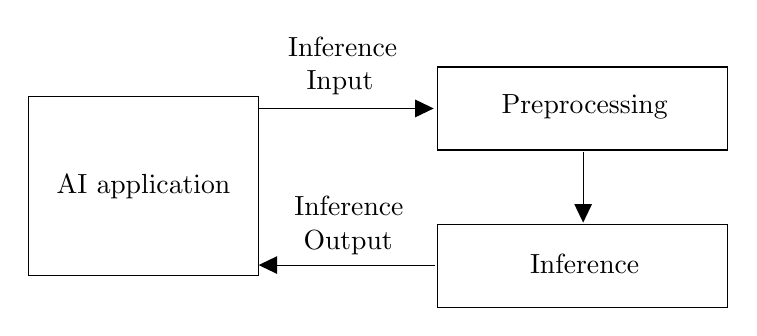
\begin{tikzpicture}[x=0.75pt,y=0.75pt,yscale=-1,xscale=1]
%uncomment if require: \path (0,300); %set diagram left start at 0, and has height of 300

%Shape: Rectangle [id:dp7725979857917211] 
\draw  [fill={rgb, 255:red, 255; green, 255; blue, 255 }  ,fill opacity=1 ] (262,80) -- (402,80) -- (402,120) -- (262,120) -- cycle ;
%Shape: Rectangle [id:dp3208391580840302] 
\draw  [fill={rgb, 255:red, 255; green, 255; blue, 255 }  ,fill opacity=1 ] (262,156) -- (402,156) -- (402,196) -- (262,196) -- cycle ;
%Straight Lines [id:da5532652572924177] 
\draw    (175.93,99.98) -- (258.29,99.98) ;
\draw [shift={(260.29,99.98)}, rotate = 180] [fill={rgb, 255:red, 0; green, 0; blue, 0 }  ][line width=0.75]  [draw opacity=0] (8.93,-4.29) -- (0,0) -- (8.93,4.29) -- cycle    ;

%Straight Lines [id:da9616587358279531] 
\draw    (332.29,121) -- (332.29,152.98) ;
\draw [shift={(332.29,154.98)}, rotate = 270] [fill={rgb, 255:red, 0; green, 0; blue, 0 }  ][line width=0.75]  [draw opacity=0] (8.93,-4.29) -- (0,0) -- (8.93,4.29) -- cycle    ;

%Straight Lines [id:da0888724954521467] 
\draw    (260.93,175.43) -- (177.93,175.43) ;
\draw [shift={(175.93,175.43)}, rotate = 360] [fill={rgb, 255:red, 0; green, 0; blue, 0 }  ][line width=0.75]  [draw opacity=0] (8.93,-4.29) -- (0,0) -- (8.93,4.29) -- cycle    ;

%Shape: Rectangle [id:dp6392688617606377] 
\draw  [fill={rgb, 255:red, 255; green, 255; blue, 255 }  ,fill opacity=1 ] (64.93,94.43) -- (175.93,94.43) -- (175.93,180.43) -- (64.93,180.43) -- cycle ;

% Text Node
\draw (333,99) node  [align=left] {Preprocessing};
% Text Node
\draw (333,175) node  [align=left] {Inference};
% Text Node
\draw (120.43,137.43) node  [align=left] {AI application};
% Text Node
\draw (216.43,79.43) node  [align=left] {Inference\\ \ \ Input};
% Text Node
\draw (219.43,156.43) node  [align=left] {Inference\\ \ Output};


\end{tikzpicture}
\caption{Visualisation of the inference process including preprocessing}
\label{fig:InfProcess}
\end{figure}
Note that the architecture of the inference model is often slightly different from the training model, as some operators are only needed for the training process and are thus removed for inference (e.\,g. dropout).






\subsection{Quantization}
\label{chap:quant}
Quantization is a technique that trades in model precision for better inference latencies, memory consumption during inference and model sizes.
Quantization describes the process of reducing the "precision representations of weights and, optionally, activations" \cite{tfLiteQuant} from floating point precision to for example 8-bit.
The weights/activations are either quantized after training the model with floats (Post Training Quantization) or the model is training with quantized weights/activations from the start (Quantization Aware Training). In the paper "Quantizing deep convolutional networks for
efficient inference"\cite{Quantizing} Krishnamoorthi performed a study on these technique with the following results:
8-bit quantization can lead to a model size reduction by a factor of 4, a 2-3x latency speedup on CPUs and DSPs, while reducing the model accuracies by 1\%.


\section{Deployment of Deep Learning Models}
Deep learning deployment describes the process of deploying a trained machine learning model to a production environment for inference purposes. 

%%Write more here
There can be differentiated in two different deployment methods, the first one is deploying the model directly to edge devices, while the second outsources the model to a cloud-backend, where the inference is performed and the prediction is then sent back to the edge device.
\subsection{Edge Deployment}
Edge deployment describes the process of deploying deep learning models to edge devices such as mobile devices like smartphones, cars or Raspberry Pis
These edge devices are characterized by offering a limited amount of hardware specifications such as amount of available energy, memory and overall computational power.
This limited power often stands in contrast to the performance demands caused real-time AI applications using deep learning models.
Despite its limits, edge deployment also has some advantages, particular in reliability and security. 
For example in the case of image classification images are needed for the inference, which often contain sensible information and thus raise a data privacy/security concern.
Therefore edge deployment should be the preferred choice, if the inference performance is sufficient for the use case of real time AI applications.

In order to increase this performance various accelerators like better GPUs, TPUs or other dedicated neural network hardware components have been developed for edge devices.
%%mention NNAPI here?



\subsection{Cloud Deployment}
While the breakthroughs in deep learning are very interesting for AI applications on edge devices, the computational demand needed for edge deployment often exceeds the available power to be viable.
That is why the option of outsourcing the models to a cloud-backend has become a popular solution in the recent years.
Cloud-backends offer a huge amount of computational power, especially suitable for deep learning in the form of GPUs, TPUs, etc.


The big downside of cloud-based inference is the needed network connection, in particular for edge devices such as cars, where a reliable network connection can often not be guaranteed for example in rural areas. Hence this is not a viable solution for applications like autonomous driving, where continuous and reliable predictions from deep learning models as critical for the.

While for the edge deployment necessary preprocessing steps are always done on the edge, for the case of cloud inference there a two possibilities. Either the input data is preprocessed to the correct shape before getting sent to the cloud-backend, or the input is sent un-preprocessed to the cloud. 
In the latter case the input gets preprocessed on the cloud. 
This can be justified by the same reasons as for the cloud inference, more computational power for intensive preprocessing.
Although slow network connection could diminish the speed up gained by the larger computational power, since non preprocessed input are most of the times larger in payload size and therefore more data has to be sent to the server, resulting in the need of faster network connections to achieve the same network latency as a preprocessed input would.
However in the case of compressed inputs as for example \emph{JPEG} images, if the \emph{JPEG} and the preprocessed image have the same input size, the \emph{JPEG} image could lead to faster latencies, as less data has to be sent to the server and the I/O overhead at the server is minimized, as the server has to load a smaller image into memory assuming \emph{JPEG} decoding is faster than the I/O overhead of load a larger image. 



\section{Inference Framework}
For both edge and cloud inference the underlying inference framework is important for the inference performance, since optimized model operations or support of accelerators like GPUs can lead to significant performance improvements.
New hardware components like accelerators and new deep learning operations for example in the form of new activation functions are being developed at fast pace, therefore a well maintained and frequently updated framework is critical for the best inference performance possible.
Another challenge is the support of the wide variety of different types of edge devices with different system architectures.

An additional factor for cloud inference affecting performance is the network component and its impact on latency.
Thus frameworks should implement low latency protocols with small payloads for environments with constrained networks.

In this thesis we only evaluate the inference performance of a single client sending requests to a cloud-backend, but in reality most of the time each edge device does not have exclusive access to a cloud-backend, resulting in multiple client making inference request to a single server, possibility even at the same time.
This raises questions on how to handle multiple requests coming from multiple sources in general and specifically how to handle multiple simultaneous requests and which requests should be prioritized.

Possible solutions include combining multiple requests and performing inference of multiple requests at once by combining them into a single batch.
This approach requires a policy on how many request to combine at most and how long the interval is where the server waits on incoming requests, if the optimal batch size is not yet reached. 
While this approach can increase throughput, it often comes at the cost of increased latency, thus negatively affecting the performance of real-time AI applications at the edge.

%%reduce data consumption?
%%REST vs gRPC
%%cloud inference needs to support multiple client-> low latency vs throughput
%%


After analyzing the problem space of deep learning inference for real-time AI applications on edge devices we can propose a performance model, that maps the aspects of the problem space on the metrics essential for assessing the performance.
	\chapter{Methodology}
In this section a performance model for understanding the runtime characteristics of deep learning models is outlined. To understand these characteristics, the underlying factors that affect it need to be understood first. 


\section{Problem Space}
The inference performance of a deep learning model is mainly affected by two major parts, the structure of the model itself and the hardware environment where it gets deployed. A third factor is the serving framework.

\subsection{Deployment}
Model deployment describes the process of deploying a trained machine learning model to a production environment for inference purposes. 

There can be differentiated in two different deployment methods, the first one is deploying the model directly to edge devices, while the second outsources the model to a cloud-backend, where the inference is performed and the prediction is sent back to the edge device.
\subsubsection{Edge Deployment}
Edge devices are characterized by offering a limited amount of hardware and are often mobile, which results in a limited amount of available energy, memory and overall computational power.
Example devices are smartphones, cars or Raspberry Pis.
Despite its limits, edge deployment also has some advantages, particular in reliability and security. 
For example in the case of image classification images are needed for the inference, which often contain sensible information and thus raise a data privacy/security concern.
Therefore edge deployment is preferred, if the inference performance is sufficient.

In order to increase this performance various accelerators like better GPUs, TPUS or other dedicated neural network hardware components have been developed for edge devices.

\begin{itemize}
    \item Was ist Edge (Beispiele)
    \item Was macht Edge aus?
\end{itemize}
\subsubsection{Cloud Deployment}
While the breakthroughs in deep learning is very interesting for AI applications on the edge devices, the computational demand needed for edge deployment often exceeds the available power to be viable.
That is why the option of outsourcing the models to a cloud-backend has become a popular solution in the recent years.
Cloud-backend offer a huge amount of computational power, especially suitable for deep learning in the form of GPUs,TPUs, etc..


The big downside of cloud-based inference is the needed network connection, in particular for edge devices such as cars, where a reliable network connection can often not be guaranteed for example in rural areas. Hence this is not a viable solution for applications that are critical like autonomous driving.
\begin{itemize}
    \item Was ist cloud?
    \item Was macht cloud aus
\end{itemize}

\subsection{Deep Learning}
Deep learning models are defined as neural networks with many layers and hidden units, the most popular being convolutional neural networks and recurrent neural networks right now, which are special forms of neural networks.
There are many different operators, which makes performance prediction very complex.
In the following the two most popular networks get analyzed.
%This increased amount of layers leads to complex mathematical calculations.

\begin{itemize}
    \item layer
    \item hidden units
    \item input size
    \item quantisation
\end{itemize}
\subsubsection{Convolutional Neural Network}
This special subclass of neural network achieved wide success in the field of object recognition and detection in images. Convolutional Neural Networks (CNN)
\paragraph{Input}
The input of CNNs often consists of images, but also can be...

\paragraph{Operations}
filter, pool, 
\subsubsection{Recurrent Neural Network}
%%%WIRKLICH MACHEN ODER NUR CNNs?
Recurrent neural networks (RNN) are made for the processing of sequences and made a lot a progress in the fields of voice recognition.
\paragraph{Input}
seqeuences
\paragraph{Operations}
GRU, LTSM
\begin{itemize}
    \item parameter von Modellen
    \item Was für Einfluss haben diese Parameter?
\end{itemize}


\section{Performance Model}
All the aspects of both hardware and model have impact on the performance, thus are the inputs of the performance model (see figure \ref{fig:perfmodel}). These input affect various performance metrics, of which inference time and throughput are the most important ones for realtime AI applications. But as the hardware on edge devices is limited and most of the times many applications need to run in parallel, low usages of the other metrics are vital as well.
\begin{figure}[H]
\centering
\includegraphics[width=0.9\textwidth]{./Bilder/trade_offs.png}
\caption{Performance Model}
\label{fig:perfmodel}
\end{figure}
\subsection{Performance Metrics}
Several metrics are important to measure the inference performance.
\subsubsection{Inference Time}
Inference time describes the time needed from requesting a prediction from a deep learning model given an specific input until getting the prediction.
This metrics is essential for the performance, since AI application often need predictions in realtime.
\subsubsection{Energy Consumption}
This metric is particular important for mobile edge devices, since they often are powered by batteries with a limited lifespan. So if the inference process of a model consumes too much energy, the application using the model is not viable.
\subsubsection{CPU Usage}
Since the inference operation is most of the time not the only process running on a system and other processes need to run simultaneously to the inference, the CPU usage is an important metric.
\subsubsection{Memory Usage}
Similar to CPU usage, inference should not occupy the whole memory of system or even demand more memory than the available memory of a edge devices.
\subsubsection{GPU Usage}
If a GPU or a another accelator is available their usage is of interest.
\subsubsection{Throughput}
In order to accomplish realtime AI a high enough throughput is essential. Therefore the number of processed predictions per second is a valuable metric.
\begin{itemize}
    \item Unterschiede aus verschiedenen deployment optionen
\end{itemize}


\endinput 
	\chapter{Methodology}
%%WHAT Is inference3
\label{chap:methodology}

In this section we present a methodology to create a decision model supporting the optimal selection of edge and cloud inference for real-time AI applications.
This methodology consists of a multi-step process and can be seen in figure \ref{fig:Methodology}, which this section will dissect into the individual steps.


\begin{figure}[!htb]
\centering
\includegraphics[width=0.96\textwidth]{./Bilder/Methodology.pdf}
\caption{Methodology to help with the optimal selection of cloud and edge inference for real-time AI applications.}
\label{fig:Methodology}
\end{figure}


In order to model the performance of deep learning inference, it is crucial to understand the underlying problem space in a first place.
Therefore all factors influencing the inference performance need to be examined.

Based on the understanding of the problem space the performance metrics then can be derived, which are critical for assessing the inference performance of a deployment option.

The net step is to design an example use case, including real world workload and infrastructure, that is used to illustrate the trade-offs between edge and cloud inference for better system understanding.


After defining the infrastructure, workload and performance metrics a benchmark system can be implemented as a framework for handling workload simulation, performance metrics instrumentation and data collection of the measurements.

Afterwards the collected measurements can be used to evaluate the trade-offs between edge and cloud deployment.
Depending on these trade-offs concrete recommendations can be given for the optimal deployment option in regard to the benchmarked infrastructure and workload.




Using the results of the evaluation and the gained system understanding we then can create a generic decision model for the deployment of deep learning models.
This decision model models the process of deciding whether a deep learning model should be deployed to the edge or to the cloud, not only for the instantiated use case, workload or infrastructure, but as a generic decision model.




%In the next section, we instantiate the presented methodology 



%In order to model the performance of deep learning inference, it is crucial to understand the underlying problem space. 
%In section \ref{chap:fundamentels} we presented the fundamentals of Deep Learning Models, their deployment and the frameworks needed to perform the inference.







\endinput 
	\chapter{Conclusion}
\label{chap:conclusion}
%kleine modelle edge, große cloud
%impact of preprocessing
%effect of NNAPI
%results mit related work vergleichen
%
\section{Future Work}
Ideen:
\begin{itemize}
    \item mix cloud/edge großen/kleinen modellen
    \item prediction of performance using the data of this thesis
\end{itemize}
\paragraph{Inference Performance Prediction}
Use data of this thesis for a machine learning model that predicts the optimal deployment solution
\paragraph{Mixed Inference}
An idea for a future study would be the combination of both cloud and edge inference to a mixed inference method for use cases of continuous inference.
This would combine both the advantages of both cloud and edge inference, as fast continuous predictions could be provided by a relatively small model on the edge device, and high accuracy predictions could be delivered by a large model hosted on a cloud-backend if demanded. 

Two event could trigger the start of the cloud inference: 
Either the edge device sends requests in periodic intervals to the cloud-backend, where the model accuracy is higher, to verify the prediction of the model on the edge devices.

The second event would be triggered by a change in prediction on the edge device. If the prediction of the edge model changes after predicting the same class/value for a extended period of time, a request could be made to the cloud-backend for reassurance. For this approach a threshold for triggering the cloud inference would be needed (e.\,g. difference between the prediction at time $t$ and the prediction at time $t-1$).



\paragraph{Retraining}
A challenge not covered in this theses  is the retraining of the model. After the model is used in production, delivering inference predictions, new training data is available. This data can be used to retrain the model to achieve higher accuracy of the model and maybe account for a concept drift, since in a dynamic environment the data distribution changes continuously.
In case of edge inference these models often get deployed to multiple edge devices with the same use case, in most cases it is more efficient to retrain the model on a cloud-backend, using the new data of all edge devices with the same use case. Another reason to retrain on the cloud is that retraining is most of the time even more computational intensive than the inference.
In the case of cloud inference, this retraining would be easier, as the data of the many clients is already at the cloud, where it can be collectively be used to retrain the network(although some privacy issues may occur).
Note that the ground truth labels for the new data needs to acquired at some point in order to retrain a model in the case of supervised learning.
\endinput 

	\chapter{Conclusion}
\label{chap:conclusion}

This thesis presented a methodology for performance evaluation of deep learning inference to support the optimal selection of deployment options for deep learning inference.

Step by step we instantiated this methodology, started by an analysis of the problem space and with it the definition of according performance metrics, followed by the design of a benchmark framework supporting real-life workloads, infrastructure and thus simulating an AI application.
We then executed this framework with 113 different parameters configurations to generate around $1700$ benchmarks.

Evaluation shows, that edge inference can achieve a better inference performance than cloud inference, at least for deep learning models with smaller architectures like MobileNetV2.
This better performance is characterized by lower latencies and higher throughput while having little to no negative impact on CPU and memory compared to cloud inference.

Furthermore, our results show the potential of model optimization techniques like quantization, as these techniques can reduce the latencies of these models by a significant factor, with little impact on accuracy.
Therefore it can be stated that these model optimization techniques should be considered for model deployment and will probably be improved even more in the near future.
%edge inference prefered because of security and netowrk

While we come to the conclusion that edge inference can provide better performance for small models, the benchmarked hardware components at the edge do not provide enough computational power for high inference performance of larger deep learning models like InceptionV4.
Therefore cloud inference is the preferred choice for large deep learning models, at least for the moment.
Also, if edge inference and cloud inference achieve the same performance, edge inference should be the favored choice as no network connection is needed and fewer data privacy concerns apply.

We believe that in the near future edge inference will be the preferred option for most model sizes, as new hardware components, inference frameworks and model optimization techniques are being developed and released.
For many future scenarios edge inference will be instrumental (e.\,g. autonomous driving) as more AI applications and edge devices are emerging.


Furthermore, we evaluated the impact of preprocessing on inference performance, resulting in the conclusion that preprocessing of large images can even take up more resources than the actual inference process does, hence becoming the bottleneck for high throughput applications.
Hence a key aspect in model deployment is the minimization of preprocessing.

Our performance model made the first step towards predicting the optimal deployment option given the system configuration and showed considerable accuracy, given the usage of a simple multiple linear regression trained with to some extent small training sets.
This performance model can be enhanced to model not only the inference performance of image classification models but deep learning models in general.

Based on this system understanding we then finally proposed a decision model for the deployment of deep learning models for inference purposes. The rationale behind this model is to deploy deep learning models to the edge if the performance is sufficient, with cloud deployment being the back-up option, as edge deployment raises fewer concerns regarding network and security.

%On key lesson
This thesis contributed a methodology for performance evaluation of deep learning inference, including the design and execution of a benchmark framework for evaluation of edge and cloud inference deployment options, and the design of a performance model utilizing the resulting benchmarks.
This framework and performance model can easily be extended to support different types of hardware and deep learning models and thus can be used as a baseline for future research on the topic of edge and cloud inference.

The goal of this thesis was to get a better understanding of deep learning inference and in particular a qualitative and quantitative investigation of different edge and cloud deployment options.
This goal was fulfilled, as the results of the instantiated methodology illustrate the trade-offs between edge and cloud inference, but also in deep learning inference in general.

%ability to instrument down to latency, CPU and memory level.


%Therefore this thesis can be concluded
\section{Future Work}
While we conducted an extensive empirical study on the trade-offs between edge and cloud inference, there are still many aspects not covered in this thesis or new research directions inspired by our results. 
In this section, we present possible ideas for future work.

\paragraph{More Benchmarks}
Due to the time constraints of this thesis, only a limited number of hardware, deep learning models and inference frameworks have been benchmarked, but the designed benchmark framework can easily be extended.


There are a wide variety of emerging edge devices with different hardware components developed towards edge inference such as FPGAs, Edge TPUs or other AI chips \cite{AItrends}.
All of these accelerators have its own unique characteristics, hence the impact of each component on inference performance needs to be studied.
This thesis studied image classification models, but the deep learning field consists of many more model types with different operators with different performance characteristics.
Examples for other popular types are object detection models, recurrent neural networks and generative adversarial networks.
Benchmarking different configuration of all these factors would help in getting an even better and more general understanding of deep learning inference.


\paragraph{Enhance Performance Model}
The performance model can be enhanced in various ways, as our performance model used simplifications, which reduced the number of factors to only two.
To generate a performance model that take these additional factors into account, more benchmarks with different configurations of these factors needs to be executed.

To make this performance model applicable to various types of deep learning model, a metric describing the complexity of the model such as number of parameters has to be developed.
The difficulty in the definition of such metrics is, that different neural network types behave very different, as they use different operators like LTSMs with different impact on performance. 
This makes generally applicable metrics very hard to define.

However the advantages of such metrics, if they are expressive enough, is that the performance of unknown deep learning models can be predicted, as long as their characteristics are known.
\paragraph{Mixed Inference}
An idea for a future study would be the combination of both cloud and edge inference to a mixed inference method for use cases of continuous inference.
This would combine both the advantages of both cloud and edge inference, as fast continuous predictions could be provided by a relatively small model on the edge device, and high accuracy predictions could be delivered by a large model hosted on a cloud-backend if demanded. 

While edge inference happens continuously, cloud inference can be triggered by two types of events:
Either the edge device sends requests in periodic intervals to the cloud-backend, where the model accuracy is higher, to verify the prediction of the model on the edge devices.
The second trigger factor could be started by a change in the edge inference predictions. If the prediction of the edge model changes after predicting the same class/value for an extended period of time, a request could be made to the cloud-backend for reassurance. For this approach a threshold for triggering the cloud inference would be needed (e.\,g. the difference between the prediction at time $t$ and the prediction at time $t-1$).



\paragraph{Retraining}
A challenge not covered in this thesis is the retraining of the model. After the model is used in production, delivering inference predictions over a period of time, new training data is available. This data can be used to retrain the model to achieve higher accuracy of the model and maybe account for a concept drift since in a dynamic environment the data distribution changes continuously.
In case of edge inference these models often get deployed to multiple edge devices with the same use case, in most cases it is more efficient to retrain the model on a cloud-backend, using the new data of all edge devices with the same use case. Another reason to retrain on the cloud is that retraining is most of the time even more computationally intensive than the inference.
In the case of cloud inference, this retraining would be easier, as the data of the many clients are already at the cloud, where it can be collectively be used to retrain the network (although some privacy issues may occur).
Note that the ground truth labels for the new data need to be acquired at some point in order to retrain a model in the case of supervised learning.

\subparagraph{Federated Learning}
One approach for retraining deep learning models on edge devices is federated learning.
Federated learning decentralizes the training of deep learning models by distributing the learning process over edge devices  \cite{federateLearning,DBLP:journals/corr/KonecnyMYRSB16}.
After a model is deployed to the edge for some time, the collected data is used to retrain the model on the edge device and results in an updated deep learning model. 
An encrypted summary of this update is then sent to a cloud-backend, where it is averaged with the updates from other edge devices to improved a shared model.
The advantage of this approach that all data stays on the edge devices, hence reducing privacy concerns.
For the benchmark framework to support federated learning the collection of training data, the training itself and communication with the shared model need to be implemented.
\endinput 

	\appendix
\chapter{Appendix}
%\section{Additional Results}
%In this Appendix one can find additional plots of the benchmarks as well as tables with details about the benchmark measurements.
\begin{figure}[!htb]
\centering
\includegraphics[width=0.71\textwidth]{./Bilder/single_plots/edge_vs_cloud_plots/Edge_vs_Cloud_Inference_Preprocessing_CPU.pdf}
\caption[Edge vs. Cloud Inference: $CPU_{preprocessing}$ - lower is better]{Edge vs. Cloud Inference: $CPU_{preprocessing}$ - lower is better - 
All $CPU_{preprocessing}$ usages are around $12.5\%$, cloud inference with cloud preprocessing having tendencies to a slightly lower usage.}
\label{fig:CloudEdgePreproCPU}
\end{figure}

\begin{figure}[!htb]
\centering
\includegraphics[width=0.71\textwidth]{./Bilder/single_plots/edge_vs_cloud_plots/Edge_vs_Cloud_Inference_Inference_Latencies_WITHOUT_NETWORK.pdf}
\caption{Edge vs. Cloud Inference: $Latency_{inference}$ without $Latency_{network}$ - lower is better - The network has little impact on the total inference latency.}
\label{fig:CloudEdgeInfLatWONetwork}
\end{figure}








\begin{figure}[!htb]
\centering
\begin{subfigure}[b]{0.95\textwidth}
   \includegraphics[width=1\linewidth]{./Bilder/single_plots/batch_size_plots/Effects_of_Batch_size_Received_Data.pdf}
   \caption{$Data_{received}$}
   \label{fig:BatchSizeReceivedData} 
\end{subfigure}

\begin{subfigure}[b]{0.95\textwidth}
   \includegraphics[width=1\linewidth]{./Bilder/single_plots/batch_size_plots/Effects_of_Batch_size_Transmitted_Data.pdf}
   \caption{$Data_{transmitted}$}
   \label{fig:BatchSizeTransmittedData}
\end{subfigure}

\caption{Edge vs.  Cloud Inference for larger Batch Sizes:  $Data_{received}$ vs. $Data_{transmitted}$ - lower is better - Increasing batch and image sizes result in more data transmitted and received.}
\end{figure}


\begin{figure}[!htb]
\centering
\begin{subfigure}[b]{0.95\textwidth}
   \includegraphics[width=1\linewidth]{./Bilder/single_plots/batch_size_plots/Effects_of_Batch_size_Inference_server_lat.pdf}
   \caption{$Latency_{server}$}
   \label{fig:BatchSizeServer} 
\end{subfigure}

\begin{subfigure}[b]{0.95\textwidth}
   \includegraphics[width=1\linewidth]{./Bilder/single_plots/batch_size_plots/Effects_of_Batch_size_Inference_network_lat.pdf}
   \caption{$Latency_{network}$}
   \label{fig:BatchSizeNetwork}
\end{subfigure}

\caption{Edge vs.  Cloud Inference for larger Batch Sizes:  $Latency_{server}$ vs. $Latency_{network}$ - lower is better - While server latency increases over rising image and batch sizes, network latency stays nearly constant.}
\end{figure}



%Add not so important result figures here%
%Table with the metrics
%\begin{table}[]
\centering
\caption{Overview of performance metrics}
\label{table:metricOverview}
\begin{tabular}{@{}ll@{}}

\toprule
\multicolumn{2}{c}{Metric}  \\
\midrule
Time & \begin{tabular}[c]{@{}l@{}}Time_{inference}\\ Time_{preprocessing}\\ Time_{total}\end{tabular} \\
Throughput & \begin{tabular}[c]{@{}l@{}}Throughput_{inference}\\ Throughput_{preprocessing}\\ Throughput_{total}\end{tabular} \\
Memory Consumption & \begin{tabular}[c]{@{}l@{}}Memory_{inference}\\ Memory_{preprocessing}\end{tabular} \\
CPU Usage & \begin{tabular}[c]{@{}l@{}}CPU_{inference}\\ CPU_{preprocessing}\end{tabular} \\
GPU Usage & \begin{tabular}[c]{@{}l@{}}GPU_{inference}\\ GPU_{preprocessing}\end{tabular} \\
Energy Consumption & \begin{tabular}[c]{@{}l@{}}Energy_{inference}\\ Energy_{preprocessing}\end{tabular} \\
Data Consumption & \begin{tabular}[c]{@{}l@{}}Data_{transmitted}\\ Data_{received}\end{tabular}\\
\bottomrule
\end{tabular}
\end{table}
\begin{sidewaystable}


    \centering
    \caption{InceptionV4 - Averages for all Metrics including standard deviation}
\scalebox{0.345}{
\begin{tabular}{lllllllllllllllllllr}
\toprule 
 \multicolumn{6}{c}{\textbf{Parameters}}&\multicolumn{4}{c}{\textbf{Preprocessing}}&\multicolumn{7}{c}{\textbf{Inference}}&\multicolumn{2}{c}{\textbf{Preprocessing+Inference}}\\
\cmidrule(lr){1-6} \cmidrule(l){7-10} \cmidrule(l){11-17}\cmidrule(l){18-19}
                  &      &           &    &      &      & $CPU_{preprocessing}$(\%) & $Memory_{preprocessing}$(MB) & $Latency_{preprocessing}$(ms) & $Throughput_{preprocessing}$ & $CPU_{inference}$(\%) & $Memory_{inference}$(MB) & $Latency_{inference}$(ms) & $Latency_{server}$(ms) & $Throughput_{inference}$ & $Data_{transmitted}$(KB) & $Data_{received}$(KB) &  $Latency_{total}$ & $Throughput_{total}$ &  Count \\
Model & Inference on & Image Size & Batch Size & Preprocessing on & NNAPI &                           &                              &                               &                              &                       &                          &                           &                        &                          &                          &                       &                    &                      &        \\
\midrule
InceptionV4 & CLOUD & 1155x1732 & 1  & CLOUD & - &               10.3 (1.77) &                123.49 (3.41) &                   16.1 (5.11) &                 66.3 (15.28) &           9.87 (1.59) &            121.13 (1.47) &            484.5 (114.04) &          397.4 (96.48) &              2.15 (0.42) &          2465.82 (38.46) &          37.82 (5.95) &     500.6 (116.62) &           2.08 (0.4) &     10 \\
                  &      &           &    & EDGE & - &                12.3 (3.1) &                 128.96 (5.3) &                 103.7 (13.27) &                    9.8 (1.4) &           9.33 (1.69) &            121.22 (4.92) &             171.0 (14.54) &          130.4 (10.33) &              5.89 (0.54) &          1058.69 (12.03) &          18.04 (1.97) &      274.7 (19.35) &          3.66 (0.26) &     10 \\
                  &      &           & 2  & CLOUD & - &              10.64 (1.51) &               141.76 (36.98) &                    18.4 (7.5) &               122.58 (44.12) &           8.02 (0.98) &            130.72 (1.58) &             557.8 (23.66) &          515.8 (24.04) &              3.59 (0.15) &           4840.62 (0.85) &           41.66 (2.8) &      576.2 (26.33) &          3.48 (0.16) &      5 \\
                  &      &           &    & EDGE & - &              17.36 (3.09) &                139.84 (4.04) &                 119.2 (13.14) &                 16.93 (1.67) &            9.1 (2.34) &            121.72 (1.61) &             260.8 (12.72) &          216.8 (13.72) &              7.68 (0.38) &           2139.9 (56.21) &          20.75 (2.14) &      380.0 (14.98) &          5.27 (0.21) &      5 \\
                  &      &           & 16 & CLOUD & - &              12.74 (0.99) &                192.38 (31.3) &                 136.2 (11.21) &                118.11 (9.66) &          11.36 (1.49) &            196.04 (0.26) &           3377.6 (173.87) &        3253.8 (174.27) &              4.75 (0.24) &         38778.96 (15.99) &         308.26 (8.23) &    3513.8 (171.77) &          4.56 (0.22) &      5 \\
                  &      &           &    & EDGE & - &              64.22 (5.34) &               301.68 (14.77) &                 358.0 (21.39) &                 44.82 (2.58) &           9.18 (2.26) &             166.5 (1.15) &           1798.6 (173.85) &        1740.0 (176.73) &              8.97 (0.94) &         16927.24 (85.02) &        176.97 (36.56) &    2156.6 (167.33) &          7.46 (0.62) &      5 \\
                  &      &           & 32 & CLOUD & - &              14.48 (1.11) &               279.04 (14.27) &                  304.4 (8.29) &                105.19 (2.86) &          11.12 (2.73) &             272.2 (0.41) &           6649.2 (764.11) &        6522.0 (773.94) &              4.86 (0.52) &        77602.64 (195.58) &       729.97 (216.52) &    6953.6 (760.31) &          4.64 (0.47) &      5 \\
                  &      &           &    & EDGE & - &              73.26 (4.68) &               385.74 (32.55) &                 689.4 (13.09) &                 46.43 (0.88) &           8.52 (2.76) &            216.28 (0.28) &           3368.0 (517.68) &        3143.0 (561.41) &              9.66 (1.32) &        33834.04 (151.05) &         354.49 (68.4) &    4057.4 (518.89) &          7.98 (0.93) &      5 \\
                  &      & 1633x2449 & 1  & CLOUD & - &              11.64 (1.57) &                122.18 (2.23) &                   21.2 (7.89) &                53.44 (19.95) &           8.48 (1.23) &             125.78 (1.0) &             724.4 (63.07) &          634.6 (29.28) &              1.39 (0.12) &          4387.17 (54.16) &          71.91 (4.72) &      745.6 (62.12) &          1.35 (0.11) &     10 \\
                  &      &           &    & EDGE & - &               11.3 (2.36) &                 137.77 (3.9) &                 163.2 (13.13) &                  6.16 (0.48) &           8.04 (2.08) &            122.76 (3.79) &              179.8 (8.38) &           137.9 (8.66) &              5.57 (0.25) &           1059.4 (11.67) &           17.0 (1.96) &       343.0 (15.9) &          2.92 (0.13) &     10 \\
                  &      &           & 2  & CLOUD & - &               13.6 (2.25) &                129.86 (6.33) &                  38.4 (10.78) &                56.15 (18.71) &           9.54 (1.34) &            129.46 (1.38) &             924.8 (54.29) &          830.4 (31.67) &              2.17 (0.13) &          8682.08 (28.51) &          88.88 (8.74) &      963.2 (47.46) &           2.08 (0.1) &      5 \\
                  &      &           &    & EDGE & - &              22.58 (3.43) &                 154.0 (2.85) &                 175.0 (11.25) &                 11.46 (0.71) &           8.14 (1.85) &            124.48 (0.65) &              235.2 (15.3) &           186.2 (8.11) &              8.53 (0.55) &           2104.03 (0.35) &          27.59 (3.74) &      410.2 (17.02) &          4.88 (0.21) &      5 \\
                  &      &           & 16 & CLOUD & - &              15.32 (1.49) &                262.56 (5.75) &                 268.0 (16.81) &                 59.88 (3.57) &          11.06 (2.26) &            249.78 (0.82) &           5480.0 (148.59) &        5359.2 (170.27) &              2.92 (0.08) &         69234.02 (21.22) &        578.97 (36.42) &    5748.0 (148.76) &          2.79 (0.07) &      5 \\
                  &      &           &    & EDGE & - &              77.58 (5.85) &               411.84 (17.71) &                 536.0 (19.96) &                 29.88 (1.14) &           7.52 (2.44) &            171.88 (7.38) &           1398.6 (129.94) &        1349.0 (113.44) &             11.51 (0.98) &          16857.1 (33.37) &        171.19 (20.52) &     1934.6 (129.9) &           8.3 (0.52) &      5 \\
                  &      &           & 32 & CLOUD & - &               15.6 (0.55) &               362.14 (61.13) &                 519.8 (23.85) &                 61.66 (2.74) &          16.94 (3.25) &           373.48 (46.74) &         12125.4 (1407.13) &      11993.0 (1467.17) &              2.67 (0.28) &       138987.98 (332.39) &      1446.92 (367.24) &  12645.2 (1395.62) &          2.55 (0.26) &      5 \\
                  &      &           &    & EDGE & - &               79.3 (1.98) &                540.22 (55.2) &                1113.8 (41.52) &                 28.76 (1.07) &           9.08 (0.84) &            219.06 (0.57) &           2703.6 (156.62) &        2593.0 (127.32) &              11.87 (0.7) &         33707.26 (59.07) &         307.17 (26.1) &    3817.4 (191.21) &           8.4 (0.42) &      5 \\
                  &      & 2309x3464 & 1  & CLOUD & - &              10.53 (1.39) &                133.16 (2.02) &                  34.1 (14.45) &                33.98 (13.05) &           6.71 (1.94) &            132.66 (0.77) &           1236.0 (108.31) &         1129.1 (95.54) &              0.81 (0.06) &          7627.07 (49.32) &        121.37 (21.74) &    1270.1 (109.96) &          0.79 (0.06) &     10 \\
                  &      &           &    & EDGE & - &              13.42 (0.51) &                152.73 (2.97) &                 276.5 (10.21) &                  3.62 (0.14) &           6.87 (1.26) &            123.95 (3.54) &             180.6 (12.43) &          140.8 (11.14) &              5.56 (0.39) &          1064.29 (26.73) &          16.69 (3.79) &      457.1 (11.83) &          2.19 (0.06) &     10 \\
                  &      &           & 2  & CLOUD & - &              10.74 (1.44) &               185.36 (54.66) &                   56.4 (6.35) &                 35.86 (4.49) &            8.06 (2.4) &             148.9 (0.54) &           1575.4 (125.78) &         1482.0 (97.31) &               1.28 (0.1) &         15108.27 (16.91) &        140.76 (18.76) &    1631.8 (125.36) &           1.23 (0.1) &      5 \\
                  &      &           &    & EDGE & - &              24.92 (0.88) &                188.58 (2.52) &                 319.6 (20.16) &                  6.28 (0.43) &           6.96 (1.18) &            128.86 (0.54) &              230.4 (6.43) &           193.2 (5.63) &              8.69 (0.24) &          2118.12 (19.62) &          26.45 (6.17) &      550.0 (17.09) &          3.64 (0.12) &      5 \\
                  &      &           & 16 & CLOUD & - &              15.48 (0.53) &               350.12 (44.81) &                  431.2 (12.7) &                 37.13 (1.08) &          14.64 (3.38) &            366.6 (23.15) &           9361.2 (200.17) &        9261.6 (187.11) &              1.71 (0.04) &        120865.59 (99.21) &       1057.77 (89.03) &    9792.4 (204.03) &          1.63 (0.03) &      5 \\
                  &      &           &    & EDGE & - &              88.56 (2.15) &               655.44 (18.75) &                 918.8 (28.26) &                 17.43 (0.53) &            7.4 (1.96) &            172.12 (0.54) &            1320.2 (79.02) &         1276.0 (85.52) &             12.15 (0.71) &          16821.55 (4.03) &        145.95 (26.45) &     2239.0 (78.27) &          7.15 (0.25) &      5 \\
                  &      &           & 32 & CLOUD & - &              15.38 (0.52) &              556.06 (103.87) &                 892.0 (16.26) &                 35.88 (0.66) &          18.62 (3.22) &             587.7 (1.38) &         18537.8 (1816.17) &      18449.4 (1804.32) &              1.74 (0.16) &       241933.22 (457.48) &      1915.82 (433.94) &  19429.8 (1800.01) &          1.66 (0.14) &      5 \\
                  &      &           &    & EDGE & - &               89.88 (3.9) &                761.3 (30.05) &                1805.6 (50.61) &                 17.73 (0.49) &           8.64 (2.51) &            221.46 (0.18) &           2661.8 (289.27) &        2575.4 (286.99) &             12.12 (1.18) &          33666.6 (28.16) &        260.11 (11.86) &    4467.4 (293.95) &          7.19 (0.44) &      5 \\
                  &      & 299x299 & 1  & CLOUD & - &               9.16 (3.12) &                121.81 (4.05) &                    1.8 (0.79) &              666.67 (293.97) &           8.89 (1.71) &            123.19 (3.56) &               95.8 (6.51) &            62.0 (5.68) &              10.48 (0.7) &            145.39 (5.91) &           3.71 (0.86) &        97.6 (6.47) &         10.29 (0.68) &     10 \\
                  &      &           &    & EDGE & - &              10.18 (2.67) &                128.07 (3.21) &                   40.3 (8.23) &                 25.74 (5.24) &           7.94 (1.89) &            127.75 (2.81) &             172.6 (11.51) &          131.2 (12.08) &              5.82 (0.41) &          1073.74 (50.92) &           14.5 (3.33) &      212.9 (16.07) &          4.72 (0.36) &     10 \\
                  &      &           & 2  & CLOUD & - &               8.18 (2.26) &                162.14 (1.02) &                    3.0 (1.22) &               746.67 (255.6) &           8.74 (0.76) &             163.5 (0.96) &              113.6 (7.23) &            72.6 (2.51) &             17.66 (1.05) &           289.64 (14.92) &           5.82 (0.86) &       116.6 (7.57) &         17.21 (1.06) &      5 \\
                  &      &           &    & EDGE & - &               13.6 (2.47) &                133.58 (0.79) &                   49.8 (7.85) &                 40.94 (6.24) &            8.32 (1.5) &            130.24 (0.82) &             259.6 (31.44) &          216.0 (26.36) &              7.79 (0.92) &          2111.64 (15.92) &          23.97 (6.19) &      309.4 (28.92) &          6.51 (0.59) &      5 \\
                  &      &           & 16 & CLOUD & - &               6.98 (0.71) &                 172.18 (1.9) &                    6.6 (0.55) &              2438.1 (208.66) &           6.76 (1.64) &            167.62 (1.32) &             378.0 (18.55) &          335.2 (13.22) &             42.41 (1.99) &          2263.74 (14.42) &          34.29 (6.35) &      384.6 (18.09) &         41.67 (1.88) &      5 \\
                  &      &           &    & EDGE & - &                27.7 (4.0) &                193.72 (8.18) &                 132.2 (19.93) &               122.97 (16.18) &            6.96 (2.5) &            174.28 (0.41) &            1431.6 (64.89) &         1393.4 (68.26) &             11.19 (0.51) &         16855.37 (18.17) &        161.81 (20.64) &     1563.8 (63.81) &         10.25 (0.42) &      5 \\
                  &      &           & 32 & CLOUD & - &               7.58 (0.58) &                 180.8 (1.59) &                   13.4 (1.14) &             2401.76 (201.77) &           7.88 (1.35) &            173.26 (1.73) &              742.2 (29.0) &          618.6 (19.14) &             43.17 (1.71) &          4519.49 (14.31) &          60.99 (6.07) &      755.6 (29.28) &          42.4 (1.66) &      5 \\
                  &      &           &    & EDGE & - &               37.52 (6.6) &               208.18 (14.95) &                 237.4 (35.57) &               137.25 (20.61) &           8.34 (1.85) &           205.18 (41.91) &            2995.2 (207.8) &        2902.6 (215.88) &             10.73 (0.75) &         33721.81 (90.85) &         309.3 (39.07) &    3232.6 (186.63) &          9.93 (0.57) &      5 \\
                  &      & 3266x4899 & 1  & CLOUD & - &              10.83 (2.21) &                139.66 (3.31) &                  43.9 (15.04) &                 24.99 (7.51) &            7.29 (2.0) &             138.11 (0.7) &           1702.3 (131.19) &        1610.7 (133.33) &              0.59 (0.05) &         10217.54 (37.26) &        160.71 (22.23) &    1746.2 (132.16) &          0.58 (0.04) &     10 \\
                  &      &           &    & EDGE & - &              13.27 (0.68) &                183.97 (2.91) &                 430.3 (15.41) &                  2.33 (0.08) &           6.76 (1.12) &            124.46 (2.84) &              202.0 (90.4) &           129.1 (6.69) &              5.42 (1.17) &            1053.45 (0.5) &           17.16 (2.9) &      632.3 (93.34) &          1.61 (0.18) &     10 \\
                  &      &           & 2  & CLOUD & - &              12.06 (2.44) &               178.44 (10.56) &                  66.8 (18.75) &                 31.73 (8.17) &           7.76 (1.91) &            159.26 (0.39) &            2079.0 (10.79) &         1962.0 (22.53) &              0.96 (0.01) &         20270.39 (19.59) &        200.77 (17.58) &     2145.8 (19.38) &          0.93 (0.01) &      5 \\
                  &      &           &    & EDGE & - &               25.1 (0.28) &                250.78 (2.07) &                 478.8 (16.42) &                  4.18 (0.14) &           5.52 (0.53) &            130.38 (0.13) &             244.4 (12.93) &          203.8 (10.01) &               8.2 (0.44) &           2117.7 (18.34) &          24.57 (5.38) &      723.2 (17.28) &          2.77 (0.07) &      5 \\
                  &      &           & 16 & CLOUD & - &               15.8 (0.45) &               432.78 (52.93) &                 635.4 (27.87) &                 25.22 (1.17) &          16.68 (2.92) &           451.82 (22.44) &          11919.8 (659.94) &       11837.4 (643.47) &              1.35 (0.07) &        161951.09 (96.05) &      1259.64 (176.78) &   12555.2 (675.56) &          1.28 (0.07) &      5 \\
                  &      &           &    & EDGE & - &               91.4 (1.52) &               1082.6 (20.95) &                1399.8 (83.21) &                 11.46 (0.68) &           9.04 (3.92) &            168.84 (4.57) &           1438.8 (120.19) &         1245.6 (109.7) &             11.18 (0.87) &        17113.46 (397.85) &         171.06 (35.9) &    2838.6 (197.64) &          5.66 (0.38) &      5 \\
                  &      &           & 32 & CLOUD & - &              16.34 (0.51) &                  452.2 (2.8) &                1327.6 (59.94) &                 24.14 (1.07) &          19.62 (1.14) &             675.0 (81.6) &         25427.4 (1280.65) &       25262.4 (1393.0) &              1.26 (0.06) &       324878.07 (552.94) &      2972.98 (240.13) &  26755.0 (1237.25) &           1.2 (0.05) &      5 \\
                  &      &           &    & EDGE & - &               91.46 (1.7) &               1236.0 (91.82) &                2717.2 (32.59) &                 11.78 (0.14) &          11.54 (1.09) &            214.92 (0.72) &           2601.4 (113.01) &        2476.8 (121.05) &             12.32 (0.53) &          33697.88 (60.9) &         257.59 (30.7) &     5318.6 (91.13) &           6.02 (0.1) &      5 \\
                  & EDGE & 1155x1732 & 1  & EDGE & True &              12.97 (2.23) &                124.98 (4.05) &                 102.4 (15.81) &                   9.97 (1.5) &           9.41 (1.25) &            272.35 (2.85) &              236.9 (2.38) &              - &              4.22 (0.04) &                - &             - &      339.3 (16.25) &          2.95 (0.14) &     10 \\
                  &      &           & 2  & EDGE & True &              15.22 (3.45) &               165.18 (18.56) &                 123.2 (20.96) &                 16.59 (2.66) &           7.72 (2.99) &            310.02 (1.45) &              468.4 (8.85) &              - &              4.27 (0.08) &                - &             - &       591.6 (13.9) &          3.38 (0.08) &      5 \\
                  &      &           & 16 & EDGE & True &              61.78 (4.16) &                326.7 (17.04) &                 394.2 (26.53) &                 40.74 (2.87) &          97.16 (0.79) &           1396.6 (16.74) &          13832.0 (259.56) &              - &              1.16 (0.02) &                - &             - &   14226.2 (271.63) &          1.13 (0.02) &      5 \\
                  &      &           & 32 & EDGE & True &               73.4 (3.01) &               481.62 (56.14) &                 686.6 (36.38) &                 46.71 (2.38) &          97.34 (1.59) &             2282.0 (5.7) &          25783.4 (472.63) &              - &              1.24 (0.02) &                - &             - &   26470.0 (487.62) &          1.21 (0.02) &      5 \\
                  &      & 1633x2449 & 1  & EDGE & False &              12.84 (2.02) &                131.83 (4.69) &                 158.5 (21.08) &                  6.41 (0.82) &          46.03 (1.39) &           385.53 (84.49) &             988.9 (11.19) &              - &              1.01 (0.01) &                - &             - &     1147.4 (25.41) &          0.87 (0.02) &     10 \\
                  &      &           &    &      & True &              13.47 (1.34) &                 131.27 (2.2) &                 169.6 (16.24) &                  5.95 (0.58) &           9.58 (2.63) &            271.47 (1.89) &              235.2 (3.01) &              - &              4.25 (0.06) &                - &             - &      404.8 (17.55) &          2.47 (0.11) &     10 \\
                  &      &           & 2  & EDGE & True &              24.06 (1.02) &                187.62 (5.45) &                 168.8 (10.13) &                 11.88 (0.67) &            9.6 (1.44) &            312.58 (0.45) &             467.8 (11.12) &              - &               4.28 (0.1) &                - &             - &       636.6 (17.2) &          3.14 (0.09) &      5 \\
                  &      &           & 16 & EDGE & True &               72.9 (4.59) &               449.34 (10.19) &                 580.2 (41.26) &                 27.69 (2.03) &           97.5 (1.55) &            1381.2 (5.45) &          13545.0 (249.42) &              - &              1.18 (0.02) &                - &             - &   14125.2 (284.17) &          1.13 (0.02) &      5 \\
                  &      &           & 32 & EDGE & True &               81.4 (1.13) &               672.08 (37.94) &                 1080.6 (75.0) &                 29.73 (2.12) &           96.8 (1.05) &           2339.0 (20.74) &          26111.2 (532.27) &              - &              1.23 (0.03) &                - &             - &   27191.8 (500.43) &          1.18 (0.02) &      5 \\
                  &      & 2309x3464 & 1  & EDGE & True &              13.75 (0.62) &                148.58 (0.65) &                 274.4 (12.92) &                  3.65 (0.17) &           7.08 (1.57) &             273.31 (0.5) &              235.8 (2.86) &              - &              4.24 (0.05) &                - &             - &      510.2 (13.36) &          1.96 (0.05) &     10 \\
                  &      &           & 2  & EDGE & True &              24.82 (1.27) &                 220.44 (1.6) &                 304.8 (13.55) &                   6.57 (0.3) &           7.32 (1.92) &            313.68 (0.42) &             469.4 (11.46) &              - &               4.26 (0.1) &                - &             - &       774.2 (8.23) &          2.58 (0.03) &      5 \\
                  &      &           & 16 & EDGE & True &              90.74 (2.12) &               704.78 (14.91) &                 911.4 (48.61) &                  17.6 (0.93) &          96.38 (0.52) &           1400.6 (16.64) &          13690.0 (269.49) &              - &              1.17 (0.02) &                - &             - &    14601.4 (254.5) &           1.1 (0.02) &      5 \\
                  &      &           & 32 & EDGE & True &              91.16 (0.51) &                941.6 (55.68) &               1769.0 (103.64) &                 18.14 (1.03) &          97.34 (1.29) &            2322.4 (16.4) &          26017.0 (425.27) &              - &              1.23 (0.02) &                - &             - &   27786.0 (410.07) &          1.15 (0.02) &      5 \\
                  &      & 299x299 & 1  & EDGE & True &              13.01 (1.16) &                116.44 (2.71) &                  45.4 (15.89) &                25.58 (12.75) &           8.24 (2.73) &            271.95 (1.76) &              235.1 (2.81) &              - &              4.25 (0.05) &                - &             - &      280.5 (17.61) &          3.58 (0.23) &     10 \\
                  &      &           & 2  & EDGE & True &              14.98 (0.71) &               159.26 (18.72) &                   50.8 (6.94) &                   40.0 (5.8) &            9.5 (2.98) &             319.68 (1.3) &              472.0 (5.43) &              - &              4.24 (0.05) &                - &             - &      522.8 (11.69) &          3.83 (0.09) &      5 \\
                  &      &           & 16 & EDGE & True &              24.88 (6.57) &               190.48 (30.32) &                 112.8 (28.06) &               150.75 (45.49) &          93.18 (6.41) &           1340.0 (51.48) &         14382.6 (1310.51) &              - &               1.12 (0.1) &                - &             - &  14495.4 (1285.38) &          1.11 (0.09) &      5 \\
                  &      &           & 32 & EDGE & True &               44.8 (14.0) &                230.8 (36.04) &                 227.4 (55.04) &               146.06 (27.77) &          95.76 (5.73) &           2183.0 (19.87) &          25779.2 (714.62) &              - &              1.24 (0.03) &                - &             - &   26006.6 (702.39) &          1.23 (0.03) &      5 \\
                  &      & 3266x4899 & 1  & EDGE & True &              13.59 (0.51) &                180.12 (0.92) &                 430.5 (15.17) &                  2.33 (0.08) &           7.64 (1.46) &            274.18 (0.35) &              237.4 (3.44) &              - &              4.21 (0.06) &                - &             - &      667.9 (15.88) &           1.5 (0.04) &     10 \\
                  &      &           & 2  & EDGE & True &                24.9 (0.6) &                281.42 (1.41) &                 463.2 (13.94) &                  4.32 (0.13) &           6.32 (1.93) &             314.4 (0.63) &              472.6 (5.73) &              - &              4.23 (0.05) &                - &             - &      935.8 (18.09) &          2.14 (0.04) &      5 \\
                  &      &           & 16 & EDGE & True &              93.04 (0.55) &               1176.0 (73.69) &                1332.4 (46.54) &                 12.02 (0.42) &          96.38 (0.52) &           1419.0 (34.26) &          13654.4 (110.89) &              - &              1.17 (0.01) &                - &             - &    14986.8 (90.45) &          1.07 (0.01) &      5 \\
                  &      &           & 32 & EDGE & True &              92.86 (1.59) &              1493.0 (163.39) &                2659.6 (66.23) &                  12.04 (0.3) &          97.48 (1.41) &           2340.0 (17.59) &          25752.0 (432.24) &              - &              1.24 (0.02) &                - &             - &   28411.6 (432.16) &          1.13 (0.02) &      5 \\
\bottomrule
\end{tabular}}

\label{measurementsInception}
\end{sidewaystable}
\begin{sidewaystable}


    \centering
    \caption{MobileNetV2 - Averages for all Metrics including standard deviation}
\scalebox{0.345}{
\begin{tabular}{llllllllllllllllllllr}
\toprule 
 \multicolumn{6}{c}{\textbf{Parameters}}&\multicolumn{4}{c}{\textbf{Preprocessing}}&\multicolumn{8}{c}{\textbf{Inference}}&\multicolumn{2}{c}{\textbf{Preprocessing+Inference}}\\
\cmidrule(lr){1-6} \cmidrule(l){7-10} \cmidrule(l){11-18}\cmidrule(l){19-20}
                   &      &           &    &      &      & $CPU_{preprocessing}$(\%) & $Memory_{preprocessing}$(MB) & $Latency_{preprocessing}$(ms) & $Throughput_{preprocessing}$ & $CPU_{inference}$(\%) & $Memory_{inference}$(MB) & $Latency_{inference}$(ms) & $Latency_{server}$(ms) & $Latency_{network}$(ms) & $Throughput_{inference}$ & $Data_{transmitted}$(KB) & $Data_{received}$(KB) &  $Latency_{total}$ & $Throughput_{total}$ &  Count \\
Model & Inference on & Image Size & Batch Size & Preprocessing on & NNAPI &                           &                              &                               &                              &                       &                          &                           &                        &                         &                          &                          &                       &                    &                      &        \\
\midrule
MobileNetV2 & CLOUD & 1155x1732 & 1  & CLOUD & - &               9.26 (3.31) &                118.19 (3.87) &                   15.2 (4.21) &                70.44 (18.89) &           7.46 (1.47) &            114.71 (3.78) &            374.07 (31.85) &         328.73 (30.25) &            45.33 (9.35) &              2.69 (0.23) &          2433.78 (31.64) &          37.97 (6.09) &     389.27 (32.67) &          2.59 (0.22) &     15 \\
                   &      &           &    & EDGE & - &              12.87 (2.89) &                122.95 (4.42) &                105.47 (19.53) &                   9.8 (1.85) &           9.48 (1.59) &            115.73 (4.71) &            105.53 (11.48) &            69.6 (9.72) &             35.93 (6.1) &              9.57 (0.98) &           599.26 (21.09) &           10.2 (1.81) &      211.0 (27.38) &          4.81 (0.61) &     15 \\
                   &      &           & 2  & CLOUD & - &               10.1 (2.71) &               131.84 (19.75) &                   22.5 (8.49) &               103.02 (43.35) &           8.45 (2.07) &           130.72 (12.96) &             623.5 (76.74) &          578.6 (71.29) &             44.9 (8.46) &              3.25 (0.42) &           4847.06 (7.75) &           47.18 (8.2) &      646.0 (75.21) &          3.13 (0.37) &     10 \\
                   &      &           &    & EDGE & - &              18.25 (2.13) &                132.59 (2.71) &                 116.3 (34.78) &                 18.15 (3.64) &           8.89 (1.84) &            117.36 (6.44) &             165.0 (19.75) &          121.9 (18.92) &             43.1 (9.28) &             12.28 (1.45) &          1192.71 (22.66) &          14.32 (4.32) &      281.3 (37.17) &          7.21 (0.86) &     10 \\
                   &      &           & 16 & CLOUD & - &              14.16 (1.29) &               200.74 (17.69) &                 148.6 (12.37) &                108.29 (8.21) &            8.0 (2.57) &           194.27 (12.41) &           4181.3 (725.59) &        4062.3 (734.86) &           119.0 (32.03) &               3.94 (0.7) &         38852.87 (98.12) &         368.8 (63.79) &    4329.9 (730.53) &          3.79 (0.66) &     10 \\
                   &      &           &    & EDGE & - &              62.38 (6.06) &               264.57 (11.58) &                 324.4 (16.51) &                 49.43 (2.44) &           8.61 (2.73) &            141.46 (2.19) &              810.7 (44.7) &          765.6 (46.47) &            45.1 (11.46) &             19.79 (1.08) &          9470.85 (37.03) &         98.94 (18.73) &     1135.1 (47.08) &         14.12 (0.59) &     10 \\
                   &      &           & 32 & CLOUD & - &              14.76 (1.15) &               279.73 (27.52) &                 308.6 (11.89) &                103.83 (3.87) &           9.71 (4.34) &           272.02 (11.02) &           6156.5 (529.74) &        6009.5 (520.15) &          147.0 (125.85) &              5.23 (0.38) &        77543.97 (200.73) &       672.17 (113.45) &    6465.1 (528.06) &          4.98 (0.35) &     10 \\
                   &      &           &    & EDGE & - &              71.02 (3.77) &               345.15 (16.53) &                  613.0 (14.2) &                 52.23 (1.19) &            7.52 (1.9) &            168.75 (2.92) &           1829.5 (359.57) &        1786.3 (356.05) &             43.2 (9.58) &             18.13 (3.65) &         18928.58 (45.72) &        154.65 (12.35) &    2442.5 (356.34) &         13.36 (1.97) &     10 \\
                   &      & 1633x2449 & 1  & CLOUD & - &              12.05 (3.42) &                117.35 (4.71) &                   23.6 (8.96) &                48.15 (18.56) &           8.41 (2.42) &            121.55 (4.16) &            589.87 (42.93) &         544.27 (42.92) &             45.6 (8.34) &               1.7 (0.12) &          4338.03 (19.48) &         53.31 (12.97) &     613.47 (47.81) &          1.64 (0.13) &     15 \\
                   &      &           &    & EDGE & - &              13.23 (1.59) &                 132.1 (3.13) &                169.53 (21.12) &                  5.99 (0.81) &            8.51 (1.6) &             117.18 (3.7) &            106.53 (11.89) &           67.47 (7.48) &            39.07 (9.25) &              9.49 (1.02) &            591.77 (0.52) &           9.92 (1.54) &      276.07 (25.3) &          3.65 (0.34) &     15 \\
                   &      &           & 2  & CLOUD & - &              11.03 (1.87) &                136.32 (6.87) &                  32.0 (12.68) &                68.92 (19.29) &           6.91 (1.51) &           140.18 (16.04) &           1082.8 (185.46) &        1017.4 (161.86) &            65.4 (47.81) &               1.89 (0.3) &           8672.6 (16.64) &         80.55 (12.25) &    1114.8 (192.76) &           1.84 (0.3) &     10 \\
                   &      &           &    & EDGE & - &              20.75 (2.59) &                144.03 (5.72) &                 179.4 (13.73) &                 11.21 (0.88) &           8.95 (1.88) &            117.12 (1.07) &             163.1 (21.54) &          119.0 (16.73) &            44.1 (11.19) &             12.44 (1.53) &           1185.48 (9.98) &          13.47 (3.54) &      342.5 (30.02) &          5.88 (0.49) &     10 \\
                   &      &           & 16 & CLOUD & - &              15.11 (0.97) &               264.42 (21.51) &                 267.9 (22.91) &                 60.09 (4.83) &          10.05 (2.61) &           255.24 (11.89) &          7089.4 (1297.18) &       6947.6 (1270.79) &           141.8 (47.06) &              2.33 (0.45) &         69303.31 (52.01) &        600.71 (59.36) &   7357.3 (1284.01) &          2.24 (0.41) &     10 \\
                   &      &           &    & EDGE & - &              76.75 (4.32) &               355.34 (25.81) &                 537.8 (34.56) &                 29.86 (1.86) &           9.05 (2.78) &            141.36 (3.83) &             824.5 (58.03) &          769.2 (65.88) &             55.3 (13.9) &             19.49 (1.41) &         9546.99 (256.09) &        110.64 (24.31) &     1362.3 (52.99) &         11.76 (0.46) &     10 \\
                   &      &           & 32 & CLOUD & - &              15.87 (1.17) &               401.48 (31.32) &                 514.8 (21.75) &                 62.26 (2.72) &          16.04 (2.19) &           393.54 (12.18) &          10608.2 (514.35) &       10508.4 (490.21) &             99.8 (36.9) &              3.02 (0.15) &        138459.99 (52.72) &       1054.25 (67.19) &   11123.0 (517.32) &          2.88 (0.13) &     10 \\
                   &      &           &    & EDGE & - &              80.05 (3.85) &               494.33 (51.21) &                1021.0 (40.84) &                 31.39 (1.24) &           7.21 (0.91) &             170.44 (2.9) &           1840.5 (395.89) &        1796.5 (392.81) &            44.0 (10.86) &             18.11 (3.79) &          18915.8 (15.34) &        183.08 (42.23) &     2861.5 (391.0) &         11.37 (1.52) &     10 \\
                   &      & 224x224 & 1  & CLOUD & - &               9.01 (2.07) &                111.01 (5.41) &                   1.87 (0.83) &              655.56 (298.59) &          10.02 (1.59) &            112.34 (5.22) &              62.47 (6.28) &           27.47 (4.16) &             35.0 (5.44) &             16.16 (1.61) &             83.84 (0.59) &           2.17 (0.38) &       64.33 (6.38) &         15.69 (1.55) &     15 \\
                   &      &           &    & EDGE & - &              12.66 (2.23) &                116.47 (2.78) &                   37.0 (4.13) &                 27.33 (2.87) &           9.06 (1.35) &            117.08 (2.29) &            110.19 (15.57) &          70.69 (11.22) &             39.5 (7.49) &              9.24 (1.22) &           608.44 (50.59) &           9.12 (2.33) &     147.19 (16.51) &          6.87 (0.73) &     16 \\
                   &      &           & 2  & CLOUD & - &               11.0 (2.56) &                109.79 (4.19) &                    2.7 (1.16) &               890.0 (449.98) &          10.65 (1.73) &            110.53 (3.94) &              77.3 (13.09) &            39.3 (7.41) &             38.0 (9.38) &             26.55 (4.45) &           169.73 (11.54) &           3.15 (0.82) &       80.0 (12.35) &         25.54 (3.92) &     10 \\
                   &      &           &    & EDGE & - &              11.88 (2.33) &                120.75 (3.98) &                    36.7 (5.1) &                  55.55 (8.5) &           7.96 (1.81) &            119.52 (3.81) &             167.2 (23.07) &          129.1 (20.33) &             38.1 (7.64) &             12.18 (1.77) &           1195.8 (28.46) &          17.54 (3.89) &      203.9 (24.55) &          9.95 (1.31) &     10 \\
                   &      &           & 16 & CLOUD & - &               9.15 (2.89) &                 117.2 (8.67) &                    9.2 (6.61) &            2407.97 (1112.08) &            8.59 (2.1) &            115.18 (5.37) &            268.0 (105.71) &          180.0 (22.23) &            88.0 (98.41) &            65.98 (17.93) &          1372.89 (83.54) &          20.95 (4.74) &     277.2 (111.75) &        64.02 (17.61) &     10 \\
                   &      &           &    & EDGE & - &              20.61 (2.19) &                143.57 (7.29) &                  67.0 (14.06) &               249.12 (55.74) &           7.07 (2.17) &            143.43 (3.34) &             904.3 (64.65) &          860.2 (67.38) &             44.1 (8.65) &             17.77 (1.22) &          9486.51 (30.29) &        114.36 (14.38) &      971.3 (68.42) &         16.54 (1.12) &     10 \\
                   &      &           & 32 & CLOUD & - &               8.54 (1.59) &                123.37 (4.22) &                    11.4 (5.1) &             3125.06 (836.31) &           8.57 (2.87) &            119.61 (4.35) &            389.1 (153.27) &          317.2 (77.43) &             71.9 (84.8) &             89.18 (20.1) &         2698.17 (173.26) &          39.75 (8.25) &      400.5 (153.2) &        86.36 (19.31) &     10 \\
                   &      &           &    & EDGE & - &              31.22 (5.47) &               192.49 (17.86) &                 140.3 (35.11) &               240.35 (58.09) &           8.06 (2.74) &            170.69 (5.21) &           1892.9 (380.23) &        1845.3 (373.33) &             47.6 (9.74) &             17.56 (3.63) &         18939.13 (43.04) &        176.39 (28.78) &    2033.2 (396.07) &         16.31 (3.29) &     10 \\
                   &      & 2309x3464 & 1  & CLOUD & - &              11.76 (1.97) &                 129.69 (5.4) &                   37.0 (9.21) &                 29.01 (9.01) &           7.82 (2.18) &            128.83 (4.61) &           1091.2 (184.73) &         965.6 (135.42) &           125.6 (63.81) &              0.94 (0.13) &          7572.68 (33.13) &         96.58 (28.27) &    1128.2 (187.77) &           0.9 (0.12) &     15 \\
                   &      &           &    & EDGE & - &              14.03 (1.07) &                 143.59 (4.4) &                269.13 (14.15) &                   3.73 (0.2) &           8.37 (1.45) &           116.73 (10.14) &            101.53 (12.98) &            66.2 (7.95) &            35.33 (6.44) &              10.0 (1.28) &           610.04 (54.28) &           9.17 (3.08) &     370.67 (21.95) &          2.71 (0.16) &     15 \\
                   &      &           & 2  & CLOUD & - &              12.54 (2.41) &                 149.49 (7.2) &                  48.9 (12.46) &                 43.08 (9.72) &           7.97 (1.59) &            136.59 (2.26) &           2219.2 (144.64) &        2082.5 (106.66) &           136.7 (66.41) &               0.9 (0.06) &          15132.9 (22.12) &       232.66 (102.94) &    2268.1 (144.34) &          0.89 (0.06) &     10 \\
                   &      &           &    & EDGE & - &              25.26 (1.69) &                175.1 (15.02) &                 308.5 (14.57) &                   6.5 (0.31) &           8.49 (1.62) &            118.22 (4.71) &             178.9 (75.89) &           113.4 (4.22) &            65.5 (73.11) &             12.14 (2.55) &           1190.72 (19.0) &           17.22 (3.6) &      487.4 (81.81) &           4.18 (0.5) &     10 \\
                   &      &           & 16 & CLOUD & - &              15.33 (1.08) &               338.98 (44.31) &                 440.1 (28.89) &                 36.48 (2.14) &          16.99 (2.61) &           353.76 (21.08) &         14787.4 (1704.29) &      14593.9 (1671.57) &           193.5 (104.9) &              1.09 (0.12) &       121094.35 (366.52) &      1774.35 (809.21) &  15227.5 (1702.41) &          1.06 (0.12) &     10 \\
                   &      &           &    & EDGE & - &              90.56 (2.01) &               623.62 (21.26) &                 870.3 (34.49) &                 18.41 (0.75) &           8.32 (1.39) &            142.09 (5.08) &             767.9 (42.12) &          720.8 (43.79) &             47.1 (7.84) &             20.89 (1.13) &          9474.72 (64.92) &         82.71 (10.22) &     1638.2 (46.93) &          9.77 (0.28) &     10 \\
                   &      &           & 32 & CLOUD & - &              15.34 (0.46) &               570.42 (42.98) &               1016.8 (253.17) &                 32.72 (5.68) &          19.87 (0.82) &            587.07 (19.1) &         25434.7 (5475.27) &      25302.4 (5457.96) &           132.3 (44.56) &              1.31 (0.27) &       242261.36 (614.35) &      3685.36 (1476.2) &   26451.5 (5352.7) &          1.25 (0.24) &     10 \\
                   &      &           &    & EDGE & - &              89.43 (1.78) &               781.12 (78.97) &                1751.6 (72.24) &                  18.3 (0.72) &           6.71 (0.91) &             171.2 (3.72) &           1839.1 (550.68) &        1794.8 (548.21) &             44.3 (9.89) &             18.75 (5.11) &         18915.84 (38.81) &          161.0 (4.93) &    3590.7 (537.14) &          9.08 (1.28) &     10 \\
                   &      & 3266x4899 & 1  & CLOUD & - &              11.21 (1.81) &                135.21 (7.62) &                  36.33 (9.99) &                 29.54 (7.97) &           6.75 (1.92) &            133.76 (4.87) &            1417.6 (74.55) &        1310.73 (62.66) &          106.87 (32.98) &              0.71 (0.04) &         10138.96 (21.58) &        114.36 (18.82) &    1453.93 (75.05) &          0.69 (0.03) &     15 \\
                   &      &           &    & EDGE & - &              14.01 (1.39) &                 174.76 (4.4) &                 427.2 (16.35) &                  2.34 (0.09) &           8.33 (1.51) &            115.07 (4.19) &              104.8 (9.97) &           67.27 (7.08) &            37.53 (7.94) &              9.63 (0.95) &           611.09 (54.37) &          10.82 (1.65) &      532.0 (14.78) &          1.88 (0.05) &     15 \\
                   &      &           & 2  & CLOUD & - &              11.12 (2.13) &                167.25 (6.91) &                   69.0 (15.5) &                 30.19 (6.13) &             7.8 (2.5) &             147.7 (1.77) &           3163.6 (314.41) &        2946.1 (256.37) &            217.5 (89.7) &              0.64 (0.07) &         20293.51 (21.64) &        311.7 (127.12) &    3232.6 (319.79) &          0.62 (0.06) &     10 \\
                   &      &           &    & EDGE & - &              25.37 (0.91) &                242.48 (9.44) &                 469.4 (12.69) &                  4.26 (0.12) &           8.02 (1.54) &            119.94 (4.43) &             156.4 (10.98) &           112.8 (9.03) &             43.6 (9.07) &              12.84 (0.9) &          1193.15 (35.78) &           17.2 (3.42) &      625.8 (18.25) &           3.2 (0.09) &     10 \\
                   &      &           & 16 & CLOUD & - &              16.54 (0.99) &               424.36 (45.45) &                  643.3 (26.8) &                 24.91 (1.06) &          17.42 (2.52) &           395.08 (94.65) &         20506.3 (2303.05) &      20372.2 (2361.54) &            134.1 (91.1) &              0.79 (0.08) &       162311.84 (165.56) &      2294.31 (1190.8) &  21149.6 (2304.55) &          0.76 (0.08) &     10 \\
                   &      &           &    & EDGE & - &              90.71 (1.21) &               1081.8 (83.15) &                 1359.2 (53.2) &                 11.79 (0.45) &           9.34 (2.03) &           146.98 (25.26) &             800.6 (70.67) &          746.9 (60.91) &            53.7 (16.07) &             20.12 (1.76) &           9466.76 (41.4) &         88.49 (23.23) &    2159.8 (102.38) &          7.42 (0.34) &     10 \\
                   &      &           & 32 & CLOUD & - &              16.12 (0.37) &                 442.34 (3.5) &                1311.6 (34.61) &                 24.41 (0.66) &          18.58 (3.45) &           706.74 (59.92) &         31090.8 (4867.09) &      30928.8 (4839.82) &          162.0 (115.59) &              1.05 (0.16) &       325170.12 (1185.2) &     4650.36 (2277.95) &  32402.4 (4891.11) &          1.01 (0.15) &     10 \\
                   &      &           &    & EDGE & - &              91.66 (1.19) &              1210.7 (177.95) &                2624.9 (64.51) &                   12.2 (0.3) &           7.58 (1.41) &            167.03 (0.75) &           1886.4 (433.76) &        1836.3 (430.96) &            50.1 (11.07) &             17.73 (3.82) &         18914.89 (23.81) &        149.38 (12.15) &    4511.3 (405.82) &          7.14 (0.62) &     10 \\
                   & EDGE & 1155x1732 & 1  & EDGE & True &              11.58 (1.93) &                121.38 (3.58) &                101.87 (16.55) &                 10.09 (1.81) &            7.71 (1.4) &            125.45 (1.41) &               28.2 (3.36) &              - &             28.2 (3.36) &             36.04 (5.29) &                - &             - &     130.07 (16.63) &          7.81 (1.07) &     15 \\
                   &      & 1633x2449 & 1  & EDGE & False &              12.87 (1.83) &                131.65 (4.78) &                158.27 (17.24) &                  6.39 (0.71) &          13.87 (2.67) &            149.12 (3.79) &              98.6 (10.23) &              - &            98.6 (10.23) &             10.24 (1.07) &                - &             - &     256.87 (21.57) &          3.92 (0.33) &     15 \\
                   &      &           &    &      & True &              12.22 (1.86) &                128.74 (1.61) &                164.53 (17.59) &                  6.15 (0.68) &            7.76 (1.5) &             126.17 (1.5) &               26.93 (3.1) &              - &             26.93 (3.1) &               37.6 (4.4) &                - &             - &     191.47 (18.52) &          5.27 (0.51) &     15 \\
                   &      & 224x224 & 1  & EDGE & True &               9.89 (1.43) &                112.88 (2.92) &                  35.93 (9.16) &                30.29 (10.81) &           7.73 (1.37) &            125.52 (3.16) &              27.73 (3.26) &              - &            27.73 (3.26) &             36.56 (4.62) &                - &             - &        63.67 (9.4) &         16.08 (2.79) &     15 \\
                   &      & 2309x3464 & 1  & EDGE & True &               13.49 (0.9) &                144.27 (1.28) &                279.73 (15.41) &                  3.59 (0.21) &           7.89 (1.46) &            126.67 (1.32) &              27.93 (3.26) &              - &            27.93 (3.26) &             36.41 (5.72) &                - &             - &     307.67 (14.67) &          3.26 (0.16) &     15 \\
                   &      & 3266x4899 & 1  & EDGE & True &              13.45 (0.62) &                174.99 (1.21) &                 427.6 (13.95) &                  2.34 (0.08) &           7.45 (1.11) &            126.97 (1.32) &            54.73 (103.04) &              - &          54.73 (103.04) &             33.84 (9.87) &                - &             - &    482.33 (100.85) &          2.13 (0.27) &     15 \\
MobileNetV2 quant & EDGE & 1155x1732 & 1  & EDGE & True &              10.45 (2.25) &                120.56 (1.06) &                 93.73 (17.94) &                 11.03 (2.06) &           7.47 (2.01) &           121.53 (13.93) &              12.67 (1.88) &              - &            12.67 (1.88) &            80.55 (11.66) &                - &             - &      106.4 (17.65) &          9.64 (1.58) &     15 \\
                   &      & 1633x2449 & 1  & EDGE & False &              12.22 (1.67) &                128.29 (3.02) &                155.87 (14.16) &                  6.47 (0.61) &           10.69 (1.8) &            117.57 (1.43) &              88.4 (24.55) &              - &            88.4 (24.55) &             12.42 (4.56) &                - &             - &     244.27 (28.94) &          4.15 (0.51) &     15 \\
                   &      &           &    &      & True &              12.52 (1.68) &                128.34 (0.86) &                161.13 (15.47) &                  6.26 (0.62) &           8.13 (1.97) &           126.98 (17.73) &              11.13 (1.51) &              - &            11.13 (1.51) &             91.2 (11.07) &                - &             - &     172.27 (15.36) &          5.85 (0.55) &     15 \\
                   &      & 224x224 & 1  & EDGE & True &               9.13 (2.28) &                111.31 (3.01) &                   32.6 (8.03) &                 32.47 (8.12) &           8.65 (1.58) &            115.15 (2.38) &               12.4 (2.61) &              - &             12.4 (2.61) &             83.86 (16.7) &                - &             - &        45.0 (8.84) &         23.06 (4.64) &     15 \\
                   &      & 2309x3464 & 1  & EDGE & True &              13.81 (0.89) &                143.81 (1.23) &                 266.2 (11.47) &                  3.76 (0.17) &           7.47 (1.82) &             116.57 (0.6) &               11.0 (1.31) &              - &             11.0 (1.31) &            92.08 (10.67) &                - &             - &      277.2 (11.17) &          3.61 (0.15) &     15 \\
                   &      & 3266x4899 & 1  & EDGE & True &              13.25 (0.68) &                 174.68 (0.7) &                430.67 (16.43) &                  2.33 (0.09) &           7.07 (1.94) &            116.93 (0.78) &               11.2 (1.47) &              - &             11.2 (1.47) &            90.55 (10.48) &                - &             - &     441.87 (17.25) &          2.27 (0.09) &     15 \\
\bottomrule
\end{tabular}}

\label{measurementsMobilenet}
\end{sidewaystable}

\lstset{basicstyle=\scriptsize}
\begin{minipage}{\linewidth}
\begin{lstlisting}[caption = $\hat{Y}_{Edge}$ Summary, escapeinside={(*}{*)}, label=lst:edgeModelSummary]
                            OLS Regression Results                            
==============================================================================
Dep. Variable:              (*$Latency_{total}$*)   R-squared:                       0.948
Model:                            OLS   Adj. R-squared:                  0.947
Method:                 Least Squares   F-statistic:                     930.9
Date:                Fri, 08 Mar 2019   Prob (F-statistic):           3.10e-66
Time:                        09:04:09   Log-Likelihood:                -540.54
No. Observations:                 105   AIC:                             1087.
Df Residuals:                     102   BIC:                             1095.
Df Model:                           2                                         
================================================================================
                  coef      std err       t        P>|t|      [0.025      0.975]
--------------------------------------------------------------------------------
Intercept      124.1744      4.007     30.991      0.000     116.227     132.122
MobileNetV2    -39.9870      4.466     -8.953      0.000     -48.846     -31.128
InceptionV4    164.1614      4.755     34.527      0.000     154.731     173.592
ImageSize     2.554e-05   7.16e-07     35.665      0.000    2.41e-05     2.7e-05
================================================================================
\end{lstlisting}

\begin{lstlisting}[caption = $\hat{Y}_{Cloud_{EdgePrepro}}$ Summary, escapeinside={(*}{*)}, label=lst:CloudEdgePreproModelSummary]
                            OLS Regression Results                            
==============================================================================
Dep. Variable:              (*$Latency_{total}$*)   R-squared:                       0.964
Model:                            OLS   Adj. R-squared:                  0.964
Method:                 Least Squares   F-statistic:                     1378.
Date:                Fri, 08 Mar 2019   Prob (F-statistic):           1.50e-74
Time:                        09:04:09   Log-Likelihood:                -496.60
No. Observations:                 105   AIC:                             999.2
Df Residuals:                     102   BIC:                             1007.
Df Model:                           2                                         
================================================================================
                  coef      std err       t        P>|t|      [0.025      0.975]
--------------------------------------------------------------------------------
Intercept      135.7102      2.736     49.607      0.000     130.284     141.136
MobileNetV2     26.8673      2.906      9.244      0.000      21.102      32.632
InceptionV4    108.8429      3.204     33.967      0.000     102.487     115.199
ImageSize     2.436e-05   5.06e-07     48.147      0.000    2.34e-05    2.54e-05
================================================================================
\end{lstlisting}
\end{minipage}

\begin{minipage}{\linewidth}
\begin{lstlisting}[caption = $\hat{Y}_{Cloud_{CloudPrepro}}$ Summary, escapeinside={(*}{*)}, label=lst:CloudCloudPreproModelSummary]
                            OLS Regression Results                            
==============================================================================
Dep. Variable:              (*$Latency_{total}$*)   R-squared:                       0.897
Model:                            OLS   Adj. R-squared:                  0.895
Method:                 Least Squares   F-statistic:                     446.2
Date:                Fri, 08 Mar 2019   Prob (F-statistic):           3.64e-51
Time:                        09:04:10   Log-Likelihood:                -688.43
No. Observations:                 105   AIC:                             1383.
Df Residuals:                     102   BIC:                             1391.
Df Model:                           2                                         
================================================================================
                  coef      std err       t        P>|t|      [0.025      0.975]
--------------------------------------------------------------------------------
Intercept      158.6698     16.568      9.577      0.000     125.807     191.533
MobileNetV2     22.3658     18.183      1.230      0.222     -13.700      58.431
InceptionV4    136.3039     19.521      6.983      0.000      97.585     175.023
ImageSize      9.35e-05    3.2e-06     29.224      0.000    8.72e-05    9.98e-05
================================================================================
\end{lstlisting}
\end{minipage}

% ---------------------------------------------------------------
\backmatter % ab hier keine Nummerierung mehr
    \listoffigures
    % \bibliographystyle{geralpha}
    \bibliographystyle{alpha}
    \bibliography{./Bib/ross17}

\end{document}
